% Created 2024-08-28 Wed 18:28
% Intended LaTeX compiler: pdflatex
\documentclass[11pt]{article}
\usepackage[utf8]{inputenc}
\usepackage[T1]{fontenc}
\usepackage{graphicx}
\usepackage{longtable}
\usepackage{wrapfig}
\usepackage{rotating}
\usepackage[normalem]{ulem}
\usepackage{amsmath}
\usepackage{amssymb}
\usepackage{capt-of}
\usepackage{hyperref}
\usepackage{siunitx}
\author{Hankertrix}
\date{\today}
\title{Intro To Thermo Fluids Cheat Sheet}
\hypersetup{
 pdfauthor={Hankertrix},
 pdftitle={Intro To Thermo Fluids Cheat Sheet},
 pdfkeywords={},
 pdfsubject={},
 pdfcreator={Emacs 29.4 (Org mode 9.6.15)}, 
 pdflang={English}}
\begin{document}

\maketitle
\setcounter{tocdepth}{2}
\tableofcontents \clearpage
\section{Definitions}
\label{sec:org3d0dee1}

\subsection{System (sys)}
\label{sec:org9bfcd73}
\begin{itemize}
\item A system is a collection of fluid particles. It moves, flows and interacts with its surroundings by exerting a force.
\item The mass of air drawn into the compressor of a jet engine is considered a "system". The air changes its properties as it is compressed and expelled through the outlet.
\end{itemize}

\subsection{Intensive property}
\label{sec:org6ac7d14}
An intensive property is a physical quantity whose value \textbf{does not} depend on the amount of substance which was measured.

\subsection{Extensive property}
\label{sec:org470cdf7}
An extensive property is a physical quantity whose value \textbf{depends} on the amount of substance which was measured.

\subsection{Specific property}
\label{sec:orgbed7e7b}
A specific property is the intensive property obtained by dividing an extensive property of a system by its mass. For example, heat capacity is an extensive property of a system.

\subsection{State}
\label{sec:org3525031}
The condition of a system described by a set of properties.
\begin{itemize}
\item It is defined by at least \textbf{2 independent intensive} properties, which is usually pressure and volume or pressure and temperature.
\end{itemize}

\subsection{Boundary}
\label{sec:org10f3549}
The real or imaginary surface that separates the system from its surroundings.

\subsection{Surroundings}
\label{sec:orgf08b728}
The mass or region outside the system.

\subsection{Isolated system}
\label{sec:orgdbad8e8}
An isolated system is a system that \textbf{does not have any exchange} of matter or energy with its surroundings. A thermos bottle containing hot water is one example, as the hot water does not spill out and the water stays hot.

\subsection{Closed system}
\label{sec:orge0005b7}
A closed system is a system that \textbf{only exchanges energy} with its surroundings. A closed system does not exchange matter with its surroundings. A mercury thermometer is one example.

\subsection{Open system (Flow system)}
\label{sec:orge7cf891}
An open system is a system where \textbf{both matter and energy} is exchanged with its surroundings. A bacterial cell is an open system, as it takes in organic matter from its surroundings, and releases heat and waste compounds to its surroundings.

\subsection{Control volume (C.V.)}
\label{sec:org7164140}
\begin{itemize}
\item A control volume is the space enclosed by the control surface in an open system.
\item A control volume is a volume in space through which a fluid may or may not flow.
\end{itemize}

\subsubsection{Selection of a control volume}
\label{sec:org08fdeff}
\begin{itemize}
\item Make the interested point \textbf{on} the control surface, not "buried" within a control volume.
\item If possible, make the control surface \textbf{perpendicular} to the fluid velocity so that the angle is either \(\qty{0}{\degree}\) or \(\qty{180}{\degree}\).
\end{itemize}

\subsection{Control surface (C.S.)}
\label{sec:org18d6164}
\begin{itemize}
\item A control surface gives a selected region in space or boundary in an open system.
\item A control surface is a surface of a control volume.
\end{itemize}

\subsection{Equilibrium}
\label{sec:org5800c36}
Equilibrium is a state of balance, and there are no unbalanced potentials within the system.

\subsubsection{Mechanical equilibrium}
\label{sec:orgfed659f}
All forces add up to zero, or the net force on a body is zero. This occurs in systems with weights, springs, etc.

\subsubsection{Thermal equilibrium}
\label{sec:orgce738e6}
No heat transfer in a system.

\subsubsection{Chemical equilibrium}
\label{sec:orgfe59c19}
No net reaction.

\subsection{Process}
\label{sec:org92c1917}
\begin{itemize}
\item A process occurs whenever a system changes from one state to another state.
\item Need to specify \textbf{initial} and \textbf{final} state, as well as the \textbf{path}, and the \textbf{interaction} with the surroundings.
\end{itemize}

\subsection{Reversible process}
\label{sec:orgac7bd8e}
Both the system and surroundings are returned to their initial state at the end of the reverse process. It is an idealised process that doesn't happen in reality.

\newpage

\subsection{Irreversible process}
\label{sec:org5913850}
An irreversible process cannot return both the system and the surroundings to their original conditions.

\subsubsection{Factors that make a process irreversible}
\label{sec:org560d1c3}
\begin{itemize}
\item Friction
\item Unrestrained expansion of a fluid
\item Mixing of different substances
\item Heat transfer through a finite temperature difference
\item Chemical reaction
\end{itemize}

\subsection{Quasi-equilibrium process}
\label{sec:org4abd280}
\begin{itemize}
\item An idealised process where a system passes through a series of equilibrium states. Basically, the system changes extremely slowly to improve the efficiency of the system and reduce the irreversibility of the system.
\item A process during which the system remains nearly in equilibrium at all times.
\end{itemize}

\subsection{Path}
\label{sec:org41833aa}
The series of states through which a system passes during a process.

\subsection{Cycle}
\label{sec:orgf77ba57}
A sequence of processes in which the working fluid returns to its original thermodynamic state.

\subsection{Macroscopic forms of energy}
\label{sec:org755e7ba}
Macroscopic forms of energy are possessed by a system as a whole with respect to an external reference frame. Examples of such forms of energy are kinetic and potential energy.

\subsection{Microscopic forms of energy}
\label{sec:orgc1855b7}
Microscopic forms of energy are related to the molecular structure and degree of molecular activity. An example of such a form of energy is internal energy.

\newpage

\subsection{Total energy (\(E\))}
\label{sec:orga0c6368}
\[E = KE + PE + U\]
\[E = \frac{1}{2} mv^2 + mgh + U\]

Where:
\begin{itemize}
\item \(E\) is the total energy
\item \(KE\) is the total kinetic energy
\item \(U\) is the internal energy
\item \(m\) is the mass of the system
\item \(v\) is the velocity of the system
\item \(g\) is the gravitational acceleration
\item \(h\) is the height of the system
\end{itemize}

\subsubsection{Change in total energy (\(\Delta E\))}
\label{sec:orgc8a0d72}
\[\Delta E = \Delta KE + \Delta PE + \Delta U\]

For a stationary, closed system:
\[\Delta E = \Delta U\]

Where:
\begin{itemize}
\item \(\Delta E\) is the change in total energy
\item \(\Delta KE\) is the change in kinetic energy
\item \(\Delta PE\) is the change in potential energy
\item \(\Delta U\) is the change in internal energy
\end{itemize}

\subsection{Internal energy (\(U\))}
\label{sec:org62d1508}
Internal energy is the sum of the energy of molecules. It is a property that includes:
\begin{itemize}
\item Molecular translation
\item Molecular rotation
\item Molecular vibration
\item Electron translation
\item Electron spin
\item Nuclear spin
\end{itemize}

\[U = U_{\text{sensible}} + U_{\text{latent}}\]

Where:
\begin{itemize}
\item \(U\) is the total internal energy
\item \(U_{\text{sensible}}\) is the sensible internal energy, which includes the internal energy from the above examples.
\item \(U_{\text{latent}}\) is the latent internal energy, which is the internal energy from the binding force between particles.
\end{itemize}

\subsection{Ice point}
\label{sec:org96abdc3}
A mixture of ice and water that is in equilibrium with air saturated with water vapour at \(\qty{1}{atm}\) pressure (\(\qty{0}{\degreeCelsius}\)).

\subsection{Steam point}
\label{sec:orgd210740}
A mixture of liquid water and water vapour with no air, in equilibrium at \(\qty{1}{atm}\) pressure (\(\qty{100}{\degreeCelsius}\)).

\subsection{Two-point temperature scale}
\label{sec:org93d49e3}
\[\frac{T - 0}{100 - 0} = \frac{X_\theta - X_0}{X_{100} - X_\theta}\]
\[T = \frac{X_\theta - X_0}{X_{100} - X_0} \times 100\]

Where:
\begin{itemize}
\item \(T\) is the current temperature
\item \(X_0\) is the value of the thermometric property at \(\qty{0}{\degreeCelsius}\)
\item \(X_{100}\) is the value of the thermometric property at \(\qty{100}{\degreeCelsius}\)
\item \(X_\theta\) is the value of the thermometric property at \(T \, \unit{\degreeCelsius}\)
\end{itemize}

\subsection{Constant volume gas thermometer}
\label{sec:org49ae7a7}
\[P = P_{atm} + h \rho g\]

Where:
\begin{itemize}
\item \(P\) is the pressure of the gas
\item \(P_{atm}\) is the atmospheric pressure
\item \(h\) is the difference in the height of the liquid between the chamber exposed to the air and the chamber exposed to the gas
\item \(\rho\) is the density of the liquid in the thermometer
\item \(g\) is the gravitational acceleration
\end{itemize}

\subsection{Pure substances}
\label{sec:org8f74651}
\begin{itemize}
\item A substance of a fixed chemical composition throughout.
\item It can have more than one \textbf{phase}, provided the chemical composition is the same (e.g. liquid water and water vapour)
\item It can be a homogenous mixture (e.g. air)
\item Non-homogeneous mixtures (e.g. oil and water) are not pure substances.
\item Homogenous mixtures with more than one phase may not be pure substances (e.g. air)
\end{itemize}

\subsection{Critical point}
\label{sec:org63c70ad}
A point at both which the saturated liquid and the saturated vapour phases are identical.

\subsubsection{Critical temperature (\(T_{cr}\))}
\label{sec:org202b72f}
The temperature at the critical point.

\subsubsection{Critical pressure (\(P_{cr}\))}
\label{sec:orge2d8427}
The pressure at the critical point.

\subsubsection{Critical volume (\(V_{cr}\))}
\label{sec:org6954e8c}
The volume at the critical point.

\subsection{Supercritical region (\(P > P_{cr} \text{ and } T > T_{cr}\))}
\label{sec:org090f97a}
The supercritical region is a region where there is no distinct phase-change process.

\subsection{Saturation temperature (\(T_{sat}\))}
\label{sec:org4af2c1d}
The temperature at which a pure substance changes phase at a \textbf{given pressure}.

\subsection{Saturation pressure (\(P_{sat}\))}
\label{sec:org32eecbb}
The pressure at which a pure substance changes phase at a \textbf{given temperature}.

\subsection{Triple point}
\label{sec:orge88accc}
\begin{itemize}
\item The triple point is the point where the three phases of a pure substance coexist in equilibrium.
\item The lines representing sublimation (solid to vapour), vaporisation (liquid to vapour), and melting (solid to liquid) meet at the triple point.
\end{itemize}

\subsection{Latent heat of fusion}
\label{sec:org8b8b638}
The energy absorbed in melting. It is equivalent to the energy released during freezing.

\subsection{Latent heat of vaporisation}
\label{sec:orgb9566d3}
The energy absorbed in vaporisation. It is equivalent to the energy released in condensation.

\subsection{Latent heat of sublimation}
\label{sec:org81ec207}
The energy absorbed in sublimation. It is equivalent to the energy released during deposition.

\subsection{Quality (dryness fraction) (\(x\))}
\label{sec:orgcb48635}
Dryness fraction, or quality, \(x\), is the proportion of \textbf{vapour} and \textbf{liquid} by \textbf{mass} in a two-phase mixture. The quality is \(0\) at the saturated liquid volume (\(v_f\)) and \(1\) at the saturated gas volume (\(v_g\)). A two-phase system can be treated as a homogenous mixture for convenience.

\[x = \frac{m_{\text{vapour}}}{m_{\text{total}}} = \frac{m_g}{m_f + m_g}\]

Where:
\begin{itemize}
\item \(x\) is the quality or dryness fraction
\item \(m_{\text{vapour}}\) is the mass of vapour
\item \(m_{\text{total}}\) is the total mass
\item \(m_g\) is the mass of vapour
\item \(m_f\) is the mass of liquid
\end{itemize}

\newpage

\subsubsection{Specific volume in terms of quality (\(v\))}
\label{sec:orgbf5a49f}
Getting the value of \(1 - x\):
\begin{align*}
1 - x &= 1 - \frac{m_g}{m_{\text{total}}} \\
&= \frac{m_{\text{total}}}{m_{\text{total}}} - \frac{m_g}{m_{\text{total}}} \\
&= \frac{m_f}{m_{\text{total}}}
\end{align*}

 \noindent Getting the specific volume in terms of quality:
\begin{align*}
v &= \frac{V_{\text{total}}}{m_{\text{total}}} \\
&= \frac{m_f v_f}{m_{\text{total}}} + \frac{m_g v_g}{m_{\text{total}}} \\
&= (1 - x) v_f + x v_g \\
&= v_f - x v_f + x v_g \\
&= v_f + x (v_g - v_f) \\
&= v_f + xv_{fg} \qquad \because v_{fg} = v_g - v_f
\end{align*}

Where:
\begin{itemize}
\item \(x\) is the quality
\item \(m_{\text{total}}\) is the total mass
\item \(m_g\) is the mass of vapour
\item \(m_f\) is the mass of liquid
\item \(v\) is the specific volume of the mixture
\item \(v_f\) is the specific volume of the liquid
\item \(v_g\) is the specific volume of the gas
\item \(v_{fg}\) is the specific volume of the mixture at evaporation
\end{itemize}

\newpage

\subsubsection{Specific internal energy in terms of quality (\(u\))}
\label{sec:orge053675}
\[u = (1 - x) u_f + xu_g = u_f + x u_{fg}\]

Where:
\begin{itemize}
\item \(u\) is the specific internal energy of the mixture
\item \(u_f\) is the specific internal energy of the liquid
\item \(u_g\) is the specific internal energy of the gas
\item \(u_{fg}\) is the specific internal energy of the mixture at evaporation
\end{itemize}

\subsubsection{Specific enthalpy in terms of quality (\(h\))}
\label{sec:org6c449bf}
\[h = (1 - x) h_f + xh_g = h_f + x h_{fg}\]

Where:
\begin{itemize}
\item \(h\) is the specific enthalpy of the mixture
\item \(h_f\) is the specific enthalpy of the liquid
\item \(h_g\) is the specific enthalpy of the gas
\item \(h_{fg}\) is the specific enthalpy of the mixture at evaporation
\end{itemize}

\newpage

\subsubsection{Quality in terms of other properties (\(x\))}
\label{sec:org455c84e}
\[x = \frac{v - v_f}{v_{fg}} = \frac{u - u_f}{u_{fg}} = \frac{h - h_f}{h_{fg}}\]

Where:
\begin{itemize}
\item \(x\) is the quality
\item \(v\) is the specific volume of the mixture
\item \(v_f\) is the specific volume of the liquid
\item \(v_g\) is the specific volume of the gas
\item \(v_{fg}\) is the specific volume of the mixture at evaporation
\item \(u\) is the specific internal energy of the mixture
\item \(u_f\) is the specific internal energy of the liquid
\item \(u_g\) is the specific internal energy of the gas
\item \(u_{fg}\) is the specific internal energy of the mixture at evaporation
\item \(h\) is the specific enthalpy of the mixture
\item \(h_f\) is the specific enthalpy of the liquid
\item \(h_g\) is the specific enthalpy of the gas
\item \(h_{fg}\) is the specific enthalpy of the mixture at evaporation
\end{itemize}

\newpage

\subsection{Enthalpy (\(H\))}
\label{sec:org66b4258}
\[H = U + PV\]

Where:
\begin{itemize}
\item \(H\) is the total enthalpy of the system
\item \(U\) is the total internal energy of the system
\item \(P\) is the pressure of the system
\item \(V\) is the total volume of the system
\end{itemize}

\subsubsection{Specific enthalpy (\(h\))}
\label{sec:org6c604b7}
\[h = u + Pv\]

Where:
\begin{itemize}
\item \(h\) is the specific enthalpy of the system
\item \(u\) is the specific internal energy of the system
\item \(P\) is the pressure of the system
\item \(v\) is the specific volume of the system
\end{itemize}

\newpage

\subsection{Van der Waals equation}
\label{sec:org81575e3}
\[\left(P + \frac{a}{v^2} \right) \left(v - b \right) = RT\]

Where:
\begin{itemize}
\item \(P\) is the pressure of the gas
\item \(a\) is related to the attraction between molecules in the gas
\item \(v\) is the molar volume, which is the total volume of the gas divided by the number of molecules of the gas
\item \(b\) is related to the size of the molecules
\item \(R\) is the universal gas constant
\item \(T\) is the current temperature
\end{itemize}

\subsubsection{Meaning of \(a\) in the equation}
\label{sec:org4784410}
\[a = \frac{27 R^2 T_{cr}^2}{64 P_{cr}}\]

Where:
\begin{itemize}
\item \(P_{cr}\) is the critical pressure of the gas
\item \(R\) is the universal gas constant
\item \(T_{cr}\) is the critical temperature of the gas
\end{itemize}

\subsubsection{Meaning of \(b\) in the equation}
\label{sec:orgd60b860}
\[b = \frac{RT_{cr}}{8 P_{cr}}\]

Where:
\begin{itemize}
\item \(R\) is the universal gas constant
\item \(T_{cr}\) is the critical temperature of the gas
\item \(P_{cr}\) is the critical pressure of the gas
\end{itemize}

\subsection{Ideal gas}
\label{sec:org60fb6e7}
The ideal gas model assumes that:
\begin{itemize}
\item The molecules are identical.
\item The molecules are in random motion.
\item The molecules obey Newton's law of motion.
\item There are \textbf{numerous molecules}.
\item The molecules are \textbf{small}.
\item There is \textbf{no intermolecular forces} between molecules.
\item Collision between molecules are \textbf{elastic}.
\item The gas is in \textbf{thermal equilibrium}, which means the temperature in every part of the gas is the same.
\item Real gases approach ideal gas behaviour when the temperature is high or the pressure is low, or low relative to temperature.
\item Real gas deviate the most from ideal gas behaviour near the critical point.
\end{itemize}

\subsection{Ideal gas laws}
\label{sec:org5812a64}

\subsubsection{Boyle's law}
\label{sec:org8027fe7}
The absolute pressure \(P\) exerted by an ideal gas is inversely proportional to the volume \(V\) if the temperature remains unchanged within a closed system.

\subsubsection{Charles' law}
\label{sec:org341bdc1}
The volume \(V\) of an ideal gas is directly proportional to its temperature \(T\) in Kelvin if pressure remains constant in a closed system.

\subsubsection{Gay-Lussac's law}
\label{sec:org912f34d}
The absolute gas pressure \(P\) is proportional to the absolute gas temperature \(T\) at constant volume in a closed system.

\subsubsection{Avogadro's law}
\label{sec:org51424cc}
Under the same conditions of temperature and pressure, equal volumes of different gases contain an equal number of molecules.

\subsection{The ideal gas equation}
\label{sec:org88ae5dd}
\[PV = nRT\]

Where:
\begin{itemize}
\item \(P\) is the pressure of the gas
\item \(V\) is the volume of the gas
\item \(n\) is the number of moles of the gas
\item \(R\) is the molar gas constant \(\qty{8.314462836}{J.mol^{-1}.K^{-1}}\)
\item \(T\) is the temperature of the gas
\end{itemize}

\subsubsection{Molar gas constant (\(R\))}
\label{sec:org2692432}
\begin{align*}
R &= N_A \times k_B \\
&= 6.02214179 \times 10^{23} \times 1.3806488 \times 10^{-23} \\
&= \qty{8.314462836}{J.mol^{-1}.K^{-1}} \\
\end{align*}

Where:
\begin{itemize}
\item \(N_A\) is Avogadro's Constant
\item \(k_B\) is the Boltzmann Constant
\end{itemize}

\subsubsection{Gas constant in terms of mass (\(R_m\))}
\label{sec:org3c59214}
\[R_m = \frac{R}{M}\]

Where:
\begin{itemize}
\item \(R_m\) is the gas constant in terms of mass
\item \(R\) is the molar gas constant
\item \(M\) is the molecular weight of a substance in \(\unit{kg.mol^{-1}}\)
\end{itemize}

\subsubsection{Compressibility factor \(Z\)}
\label{sec:orgf0da123}
\begin{itemize}
\item For ideal gases, the compressibility factor is 1.
\end{itemize}

\[Z = \frac{v_{\text{actual}}}{v_{\text{ideal}}}\]

Where:
\begin{itemize}
\item \(Z\) is the compressibility factor
\item \(v_{\text{actual}}\) is the actual specific volume of the gas
\item \(v_{\text{ideal}}\) is the specific volume of an idea gas
\end{itemize}

\[Pv = ZR_mT\]

Where:
\begin{itemize}
\item \(P\) is the pressure of the gas
\item \(v\) is the specific volume of the gas
\item \(R_m\) is the gas constant based on mass
\item \(T\) is the temperature of the gas
\end{itemize}

\subsubsection{Comparing ideal gas states}
\label{sec:org090f1e4}
\[\frac{P_1 V_1}{T_1} = \frac{P_2 V_2}{T_2}\]

Where:
\begin{itemize}
\item \(P\) is the pressure of the gas in the respective states
\item \(V\) is the volume of the gas in the respective states
\item \(T\) is the temperature of the gas the respective states
\end{itemize}

\subsubsection{Obtaining the specific heats}
\label{sec:orgbb6d293}
For an ideal gas, specific internal energy \(u\) and specific enthalpy \(h\) are functions of temperature only, i.e:
\[u = u(T)\]
\[h = u(T) + R_mT = u(T) + Pv = h(T)\]

The specific heats of ideal gases are hence functions of temperature only as well:
\[c_v = c_v(T) = \frac{du}{dT}\]
\[c_p = c_p(T) = \frac{dh}{dT}\]

Hence:
\[\Delta u = u_2 - u_1 = \int_1^2 c_v(T) \, dT \cong c_{v_{avg}} \left(T_2 - T_1 \right)\]
\[\Delta h = h_2 - h_1 = \int_1^2 c_p(T) \, dT \cong c_{p_{avg}} \left(T_2 - T_1 \right)\]

Where:
\begin{itemize}
\item \(u\) is the specific internal energy of the system
\item \(h\) is the specific enthalpy of the system
\item \(T\) is the temperature of the system
\item \(R_m\) is the gas constant based on mass
\item \(P\) is the pressure of the gas
\item \(v\) is the specific volume of the gas
\item \(T_2\) is the \textbf{final} temperature of the system
\item \(T_1\) is the \textbf{initial} temperature of the system
\item \(c_v\) is the specific heat at constant volume
\item \(c_p\) is the specific heat at constant pressure
\item \(c_{v_{avg}}\) is the specific heat at constant volume at an average temperature
\item \(c_{p_{avg}}\) is the specific heat at constant pressure at an average temperature
\end{itemize}

\subsubsection{Relations between specific heats}
\label{sec:orgff210ee}
\[c_p = c_v + R_m\]
\[c_v = \frac{R_m}{k - 1}\]
\[c_p = \frac{kR_m}{k - 1}\]

Where:
\begin{itemize}
\item \(c_p\) is the specific heat at constant pressure
\item \(c_v\) is the specific heat at constant volume
\item \(R_m\) is the gas constant based on mass
\item \(k\) is the specific heat ratio
\end{itemize}

\subsection{Virial equation}
\label{sec:orge5c254f}
The virial equation is used to describe the causes of non-ideality at a molecular level as very few gases are mono-atomic.

\[Z = \frac{Pv}{R_m T} = 1 + \frac{B(T)}{v} + \frac{C(T)}{v^2} + \frac{D(t)}{v^3} + \cdots\]

Where:
\begin{itemize}
\item \(Z\) is the compressibility factor
\item \(P\) is the pressure of the gas
\item \(v\) is the specific volume of the gas
\item \(R_m\) is the gas constant based on mass
\item \(T\) is the temperature of the gas
\item \(B, C, D\) are known as virial coefficients and are functions of temperature
\end{itemize}

\subsection{Reduced pressure (\(P_R\))}
\label{sec:org7f107b8}
\[P_R = \frac{P}{P_{cr}}\]

Where:
\begin{itemize}
\item \(P_R\) is the reduced pressure
\item \(P\) is the pressure of the gas
\item \(P_{cr}\) is the critical pressure of the gas
\end{itemize}

When reduced pressure is much smaller than 1 (\(P_R << 1\)), the gas approaches ideal gas behaviour.

\subsection{Reduced temperature (\(T_R\))}
\label{sec:org6eea2a6}
\[T_R = \frac{T}{T_{cr}}\]

Where:
\begin{itemize}
\item \(T_R\) is the reduced temperature
\item \(T\) is the temperature of the gas
\item \(T_{cr}\) is the critical temperature of the gas
\end{itemize}

When reduced temperature is greater than 2 (\(T_R > 2\)), the gas approaches ideal gas behaviour.

\subsection{Pseudo-reduced specific volume (\(v_R\))}
\label{sec:org916fe60}
\[v_R = \frac{v_{\text{actual}}}{\frac{1}{P_{cr}} \left(R_m T_{cr} \right)}\]

Where:
\begin{itemize}
\item \(v_R\) is the pseudo-reduced specific volume
\item \(v_{\text{actual}}\) is the actual specific volume of the gas
\item \(R_m\) is the gas constant based on mass
\item \(T_{cr}\) is the critical temperature of the gas
\item \(P_{cr}\) is the critical pressure of the gas
\end{itemize}

\subsection{Zeroth law of thermodynamics}
\label{sec:org0644605}
If two objects are each in thermal equilibrium with third object, then the two objects are in equilibrium with each other.

\subsection{First law of thermodynamics}
\label{sec:orgab0facf}
The first law of thermodynamics states that in any process, regardless of the process' spontaneity, the total energy of a system and its surroundings is constant.

\[E_{in} - E_{out} = \Delta E_{\text{system}}\]

Where:
\begin{itemize}
\item \(E_{in}\) is the energy input into the system
\item \(E_{out}\) is the energy leaving the system
\item \(\Delta E_{\text{system}}\) is the change in energy of the system
\end{itemize}

\subsection{Second law of thermodynamics}
\label{sec:orge2a0cd1}
The second law of thermodynamics states that in any \textbf{spontaneous} process, the total entropy of a system and its surroundings always increases.

\subsection{Third law of thermodynamics}
\label{sec:orge013d8e}
The third law of thermodynamics states that the entropy of a perfectly ordered crystalline substance at 0 K is zero.

\subsection{Heat (\(Q\))}
\label{sec:orgb7f5e7e}
\begin{itemize}
\item Heat is a means of energy transfer between a system and its surroundings as a result of a \textbf{temperature difference} between them.
\item Heat is process related (i.e. it is a path function), not a property.
\end{itemize}

Units: \(\unit{J}\) or \(\unit{kJ}\)

\subsubsection{Heat rate (\(Q\))}
\label{sec:orgdcd0368}
Heat rate is the rate of heat transferred.
\\[0pt]

 \noindent Units: \(\unit{W}\) or \(\unit{kW}\)

\subsection{Heat per unit mass (\(q\))}
\label{sec:orgd3b3e2b}
\[q = \frac{Q}{m}\]

Where:
\begin{itemize}
\item \(q\) is the heat per unit mass
\item \(Q\) is the total heat transferred
\item \(m\) is the mass of the object
\end{itemize}

Units: \(\unit{kJ.kg^{-1}}\)

\subsection{Temperature difference}
\label{sec:orgc872303}
\begin{itemize}
\item Temperature difference is the driving force for heat transfer. The larger the temperature difference, the higher the rate of heat transfer.
\item Energy is recognised as heat transfer only as it \textbf{crosses} the system boundary.
\item The larger the driving force, the higher the heat transferred.
\end{itemize}

\subsection{Conduction: Fourier's law}
\label{sec:orgc9b12e8}
\[Q_{cond} = -kA \frac{dT}{dx}\]

\subsection{Convection: Newton's law of cooling}
\label{sec:org2ba0015}
\[Q_{conv} = hA(T_s - T_f)\]

\subsection{Radiation: Stefan-Boltzmann's law}
\label{sec:org39d01c5}
\[Q_{rad} = \varepsilon \sigma A(T_s^4 - T_{surr}^4)\]

\newpage

\subsection{Work done (\(W\))}
\label{sec:orgb84cd37}
\begin{itemize}
\item Work is a means of energy transfer between a system and its surroundings. For a \textbf{closed} system, if energy transfer is not by \textbf{heat}, it must be by \textbf{work}.
\item Work is energy transfer associated with a \textbf{force} acting through a \textbf{distance}. For example, a rising piston, a rotating shaft, and electric current through a wire.
\item Work is \textbf{process} related (i.e. it is a path function), not a property.
\end{itemize}

\[W = \int_1^2 \vec{F} \cdot ds\]

Where:
\begin{itemize}
\item \(W\) is the work done
\item \(\vec{F}\) is the force acting on the system
\item \(ds\) is the length of infinitesimal element of the path taken by the force
\end{itemize}

\subsubsection{Work rate (Power) (\(P\))}
\label{sec:orge75ec9c}
\[P = \frac{W}{t}\]

Where:
\begin{itemize}
\item \(P\) is the power
\item \(W\) is the work done
\item \(t\) is the time taken for the work to be done on the system in seconds
\end{itemize}

Units: \(\unit{W}\) or \(\unit{kW}\)

\newpage

\subsubsection{Work done per unit mass (\(w\))}
\label{sec:org884b5d8}
\[w = \frac{W}{m}\]

Where:
\begin{itemize}
\item \(w\) is the work done per unit mass on the system
\item \(W\) is the work done
\item \(m\) is the mass of the system
\end{itemize}

Units: \(\unit{kJ.kg^{-1}}\)

\subsubsection{Mechanical work done (\(W\))}
\label{sec:org2309475}
Mechanical work done is the product of the force \(F\) displace a distance \(s\) in the direction of the force.

\[W = Fs\]

Where:
\begin{itemize}
\item \(W\) is the mechanical work done
\item \(F\) is the force on the system
\item \(s\) is the distance displaced by the force
\end{itemize}

When the force is not constant:

\[W = \int_1^2 \vec{F} \cdot ds = \int_1^2 F \, ds\]

Where:
\begin{itemize}
\item \(W\) is the mechanical work done
\item \(F\) is the force on the system
\item \(ds\) is the length of infinitesimal element of the path taken by the force
\end{itemize}

\newpage

\subsubsection{Boundary work (\(P \, dV\) work) (\(W_b\))}
\label{sec:org382c397}
\begin{itemize}
\item Boundary work is the work associated with a moving boundary.
\item An example is the work done by the expansion and the compression of a piston cylinder device.
\item Boundary work is \textbf{positive for expansion}, and \textbf{negative for compression}.
\item The area under the curve on a \(P - V\) diagram represents the boundary work.
\end{itemize}

\[\delta W_b = F \, ds = PA \, ds = P \, dV\]
\[W_b = \int_1^2 P \, dV\]

Where:
\begin{itemize}
\item \(\delta W_b\) is the infinitesimal change in boundary work
\item \(W_b\) is the boundary work
\item \(F\) is the force on the system
\item \(ds\) is the length of the infinitesimal element of the path taken by the force
\item \(P\) is the pressure of the system
\item \(A\) is the area of the system
\item \(dV\) is the infinitesimal change in volume of the system
\end{itemize}

\newpage

\subsubsection{Shaft work (\(W_{sh}\))}
\label{sec:org7ef635b}
\[P = W_{sh} = \tau \omega = 2 \pi f \tau\]

Where:
\begin{itemize}
\item \(P\) is the power
\item \(W_{sh}\) is the work done
\item \(\tau\) is the torque applied on the shaft
\item \(\omega\) is the angular frequency
\item \(f\) is the frequency of rotation of the shaft, or the number of revolutions per unit time of the shaft
\end{itemize}

\newpage

\subsubsection{Spring work (\(W_{\text{spring}}\))}
\label{sec:orgd1e069f}
For a linear elastic spring, the displacement is proportional to the force applied:
\[F = kx\]

Where:
\begin{itemize}
\item \(F\) is the elastic spring force
\item \(k\) is the spring constant
\item \(x\) is the displacement of the spring
\end{itemize}

The spring work is:
\[W_{\text{spring}} = \int_1^2 F \, dx = \int_1^2 kx \, dx = \frac{1}{2}k \left(x_2^2 - x_1^2 \right)\]

Where:
\begin{itemize}
\item \(W_{\text{spring}}\) is the work done
\item \(F\) is the elastic spring force
\item \(dx\) is the infinitesimal element of the path taken by the spring
\item \(k\) is the spring constant
\item \(x\) is the displacement of the spring
\item \(x_2\) is the \textbf{final} displacement of the spring
\item \(x_1\) is the \textbf{initial} displacement of the spring
\end{itemize}

For the expansion of a gas in a piston-cylinder against a spring:
\[W_{\text{linear}} = \frac{P_2 + P_1}{2} \left(V_2 - V_1 \right) = P_{avg} \Delta V\]

Where:
\begin{itemize}
\item \(P_2\) is the \textbf{final} pressure
\item \(P_1\) is the \textbf{initial} pressure
\item \(V_2\) is the \textbf{final} volume
\item \(V_1\) is the \textbf{initial} volume
\item \(P_{avg}\) is the average pressure of the final and initial pressures
\item \(\Delta V\) is the change in volume of the system
\end{itemize}

\subsubsection{Gravitational work (\(W_g\))}
\label{sec:org966d654}
\begin{itemize}
\item Gravitational work is the work done against a gravitational field.
\item It is equal to the change in gravitational potential energy of the system
\item As potential energy is dependent only on the end states, it is a property.
\end{itemize}

\[W_g = \int_1^2 F \, dz = \int_1^2 mg \, dz = mg(z_2 - z_1)\]

Where:
\begin{itemize}
\item \(W_g\) is the work done against gravity
\item \(F\) is the gravitational force
\item \(m\) is the mass of the object
\item \(g\) is the gravitational acceleration
\item \(dz\) is the infinitesimal element of the path taken by the object through a gravitational field
\item \(z_2\) is the \textbf{final} height of the object
\item \(z_1\) is the \textbf{initial} height of the object
\end{itemize}

\newpage

\subsubsection{Acceleration work (\(W_a\))}
\label{sec:orgb3ab721}
\begin{itemize}
\item Acceleration work is the work associated with the change in velocity of a system.
\item It is equal to the change in \textbf{kinetic} energy of the system.
\end{itemize}

\[W_a = \int_1^2 F \cdot ds = \int_1^2 m \frac{dv}{dt} v \, dt = m \int_1^2 v \, dv = \frac{1}{2} \left(v_2^2 - v_1^2 \right)\]

Where:
\begin{itemize}
\item \(W_a\) is the work done due to acceleration
\item \(F\) is the force
\item \(m\) is the mass of the object
\item \(\frac{dv}{dt}\) is the change in velocity with respect to time
\item \(v_2\) is the \textbf{final} velocity of the object
\item \(v_1\) is the \textbf{initial} velocity of the object
\end{itemize}

\newpage

\subsubsection{Electrical work (\(W_e\))}
\label{sec:org24d0692}
\[W_e = V_e N\]
\[W_e = \int_1^2 V_e I \, dt\]

Where:
\begin{itemize}
\item \(W_e\) is the electrical work done
\item \(V_e\) is the potential difference
\item \(N\) is the charge
\item \(I\) is the current
\item \(dt\) is the infinitesimal time element
\end{itemize}

\[P_e = V_e I\]
Where:
\begin{itemize}
\item \(P_e\) is the electrical power
\item \(V_e\) is the potential difference
\item \(I\) is the current
\end{itemize}

\subsection{Properties}
\label{sec:org5092aca}
Properties are \textbf{point} functions and are state dependent.

\subsection{Specific heat capacity (\(c\))}
\label{sec:orgb963d30}
Specific heat capacity is the energy required to raise the temperature of a unit mass of a substance by one degree Celsius.
\\[0pt]

For gases, there are:
\begin{enumerate}
\item Specific heat at constant volume, \(c_v\)
\item Specific heat at constant pressure, \(c_p\)
\end{enumerate}

\newpage

\subsubsection{Specific heat at constant volume (\(c_v\))}
\label{sec:org93e2821}
\begin{itemize}
\item The specific heat at constant volume is the energy required to raise the temperature of a unit mass of a substance by one degree while the \textbf{volume remains constant}.
\item This only applies to gases.
\item It is an intensive property and is dependent on volume \(v\) and temperature \(T\).
\end{itemize}

\[c_v = \left. \frac{\partial u}{\partial T} \right|_v\]

Where:
\begin{itemize}
\item \(c_v\) is the specific heat at constant volume
\item \(\left. \frac{\partial u}{\partial T} \right|_v\) is the partial derivative of the internal energy with respect to temperature, restricted to the constant volume \(v\)
\end{itemize}

\subsubsection{Specific heat at constant pressure (\(c_p\))}
\label{sec:org11ab1c7}
\begin{itemize}
\item The specific heat at constant volume is the energy required to raise the temperature of a unit mass of a substance by one degree while the \textbf{pressure remains constant}.
\item This only applies to gases.
\item It is an intensive property and is dependent on pressure \(P\) and temperature \(T\).
\end{itemize}

\[c_p = \left. \frac{\partial h}{\partial T} \right|_v\]

Where:
\begin{itemize}
\item \(c_p\) is the specific heat at constant pressure
\item \(\left. \frac{\partial h}{\partial T} \right|_v\) is the partial derivative of the enthalpy with respect to temperature, restricted to the constant volume \(v\)
\end{itemize}

\subsubsection{Specific heat ratio (\(k\))}
\label{sec:org4e19675}
\[k = \frac{c_p}{c_v}\]

Where:
\begin{itemize}
\item \(c_p\) is the specific heat at constant pressure
\item \(c_v\) is the specific heat at constant volume
\end{itemize}

\subsection{Internal energy change (\(\Delta U\))}
\label{sec:org7593f7c}
The internal energy change \textbf{does not} include the work done by the gas during expansion or compression.
\[\Delta u = u_2 - u_1 \cong c_v \left(T_2 - T_1 \right)\]

Where:
\begin{itemize}
\item \(\Delta u\) is the change in internal energy
\item \(u_2\) is the \textbf{final} specific internal energy
\item \(u_1\) is the \textbf{initial} specific internal energy
\item \(c_v\) is the specific heat capacity at constant volume
\item \(T_2\) is the \textbf{final} temperature
\item \(T_1\) is the \textbf{initial} temperature
\end{itemize}

\newpage

\subsection{Enthalpy change (\(\Delta H\))}
\label{sec:orgdafb664}
\begin{itemize}
\item The enthalpy change \textbf{does} include the work done by the gas during expansion or compression.
\item Use this when there is no need to calculate the work done by the gas.
\end{itemize}
\[\Delta h = h_2 - h_1 \cong c_p \left(T_2 - T_1 \right)\]

Where:
\begin{itemize}
\item \(\Delta h\) is the change in enthalpy
\item \(h_2\) is the \textbf{final} specific enthalpy
\item \(h_1\) is the \textbf{initial} specific enthalpy
\item \(c_p\) is the specific heat capacity at constant pressure
\item \(T_2\) is the \textbf{final} temperature
\item \(T_1\) is the \textbf{initial} temperature
\end{itemize}

\subsection{Energy of a system (\(E_{\text{system}}\))}
\label{sec:org73310ee}

\subsubsection{Total energy (\(E_{\text{system}}\))}
\label{sec:orge697f42}
\[E_{\text{system}} = U + KE + PE\]

Where:
\begin{itemize}
\item \(E_{\text{system}}\) is the total energy of the system
\item \(U\) is the total internal energy of the system
\item \(KE\) is the total kinetic energy of the system
\item \(PE\) is the total potential energy of the system
\end{itemize}

\newpage

\subsubsection{Change in energy (\(\Delta E\))}
\label{sec:org8bd9c69}
\[\Delta E_{\text{system}} = \Delta U + \Delta KE + \Delta PE\]

Where:
\begin{itemize}
\item \(\Delta E_{\text{system}}\) is the change in energy of the system
\item \(\Delta U\) is the change in internal energy of the system
\item \(\Delta KE\) is the change in kinetic energy of the system
\item \(\Delta PE\) is the change in potential energy of the system
\end{itemize}

For a fixed mass:
\[\Delta U = m (u_2 - u_1)\]
\[\Delta KE = \frac{1}{2} m (v_2^2 - v_1^2)\]
\[\Delta U = mg (z_2 - z_1)\]

Where:
\begin{itemize}
\item \(\Delta U\) is the change in internal energy of the system
\item \(m\) is the mass of the system
\item \(u_2\) is the \textbf{final} specific internal energy of the system
\item \(u_1\) is the \textbf{initial} specific internal energy of the system
\item \(\Delta KE\) is the change in kinetic energy of the system
\item \(v_2\) is the \textbf{final} velocity of the system
\item \(v_1\) is the \textbf{initial} velocity of the system
\item \(\Delta PE\) is the change in potential energy of the system
\item \(z_2\) is the \textbf{final} height of the system
\item \(z_1\) is the \textbf{initial} height of the system
\end{itemize}

For stationary systems, \(\Delta KE = 0\) and \(\Delta PE = 0\):
\[\Delta E_{\text{system}} = \Delta U\]

Where:
\begin{itemize}
\item \(\Delta E_{\text{system}}\) is the change in energy of the system
\item \(\Delta U\) is the change in internal energy of the system
\end{itemize}

\subsection{Conservation of mass principle}
\label{sec:orgfc2f068}
\begin{itemize}
\item For \textbf{closed systems}, the principle is implicit since the mass of a closed system is kept constant during a process.
\item For \textbf{control volumes}, mass can cross boundaries, so it is required to track the amount of mass \textbf{leaving} and \textbf{entering} the control volume.
\item The net \textbf{mass transfer} to or from a system during a process is equal to the \textbf{net change} (increase or decrease) in the total mass of the control volume.
\end{itemize}

\[\sum m_{i} - \sum m_{e} = \Delta m_{CV} = \left(m_2 - m_1 \right)_{CV}\]

Where:
\begin{itemize}
\item \(\sum m_{i}\) is the total mass entering (mass input) the control volume
\item \(\sum m_{e}\) is the total mass exiting the control volume
\item \(\Delta m_{CV}\) is change in total mass of the control volume
\item \(m_2\) is the final mass of the control volume
\item \(m_1\) is the initial mass of the control volume
\end{itemize}

\newpage

\subsection{Flow work (Flow energy) (\(W_{flow}\))}
\label{sec:orgd98f65b}
\begin{itemize}
\item The work (or energy) required to push the mass into or out of the control volume.
\item This work is necessary for maintaining a continuous flow through a control volume.
\item Flow work is the energy needed to maintain continuous flow through a control volume.
\end{itemize}

\[W_{flow} = FL = PAL = PV\]

Where:
\begin{itemize}
\item \(W_{flow}\) is the flow work
\item \(F\) is the force on the control volume
\item \(L\) is the distance acted upon by the force
\item \(P\) is the pressure due to the force
\item \(A\) is the cross-sectional area of the fluid that the force is acting on
\item \(V\) is the volume acted on by the force
\end{itemize}

\subsubsection{Specific flow work (flow work per unit mass) (\(w_{flow}\))}
\label{sec:orgdc94f0f}
\[w_{flow} = Pv\]

Where:
\begin{itemize}
\item \(w_{flow}\) is the \textbf{specific} flow work
\item \(P\) is the pressure due to the force
\item \(v\) is the \textbf{specific} volume acted on by the force
\end{itemize}

\subsubsection{Total energy per unit mass of a \emph{flowing fluid} (\(\theta\))}
\label{sec:org1097ae1}
\[\theta = Pv + e = Pv + (u + \text{ke} + \text{pe})\]

Since \(h = u + Pv\):
\[\theta = h + \text{ke} + \text{pe} = h + \frac{V^2}{2} + gz\]

For a \textbf{non-flowing} fluid:
\[e = u + \text{ke} + \text{pe}\]

For a \textbf{flowing} fluid:
\[\theta = h + \text{ke} + \text{pe}\]

Where:
\begin{itemize}
\item \(\theta\) is the total energy per unit mass of a \textbf{flowing fluid}
\item \(P\) is the pressure on the fluid
\item \(v\) is the \textbf{specific} volume of the fluid
\item \(e\) is the \textbf{specific} energy of the fluid
\item \(u\) is the \textbf{specific} internal energy of the fluid
\item \(\text{ke}\) is the \textbf{specific} kinetic energy of the fluid
\item \(\text{pe}\) is the \textbf{specific} potential energy of the fluid
\item \(h\) is the \textbf{specific} enthalpy of the fluid
\item \(V\) is the velocity of the fluid
\item \(g\) is the gravitation acceleration
\item \(z\) is the height of the fluid
\end{itemize}

\subsubsection{Net energy change in a control volume}
\label{sec:org817f28b}
\[E_{\text{mass, } i} - E_{\text{mass, } e} = m_i \theta_i - m_e - \theta_e\]

Where:
\begin{itemize}
\item \(E_{\text{mass, } i}\) is the energy input into the control volume
\item \(E_{\text{mass, } e}\) is the energy exiting the control volume
\item \(m_i\) is the mass input into the control volume
\item \(\theta_i\) is the total energy per unit mass input into the control volume
\item \(m_e\) is the mass exiting the control volume
\item \(\theta_e\) is the total energy per unit mass exiting the control volume
\end{itemize}

\subsubsection{First law of thermodynamics for a control volume}
\label{sec:org150e5af}
\[Q - W + m_i \theta_i - m_e \theta_e = \left(E_2 - E_1 \right)_{CV}\]

Where:
\begin{itemize}
\item \(Q\) is the heat supplied to the control volume
\item \(W\) is the work done by the control volume
\item \(m_i\) is the mass input into the control volume
\item \(\theta_i\) is the total energy per unit mass input into the control volume
\item \(m_e\) is the mass exiting the control volume
\item \(\theta_e\) is the total energy per unit mass exiting the control volume
\item \(E_2\) is the final total energy of the control volume
\item \(E_1\) is the initial total energy of the control volume
\end{itemize}

\subsection{Steady state}
\label{sec:org80a4791}
A steady state implies that fluid properties can be different from point to point in the control volume, but they do not change with time.

\subsection{Steady flow}
\label{sec:orgd73d605}
\begin{itemize}
\item Steady flow implies that properties at the inlet and exit may be different but do not change with time.
\item Properties at each opening are usually considered uniform.
\item Heat and work interactions also don't change with time.
\item Hence, net energy transfer across the boundary is zero.
\item A steady state is used to evaluate devices that operate for long periods of time under the same conditions (steady-flow devices).
\end{itemize}

\subsubsection{Mass balance}
\label{sec:orge459be9}
\[\frac{dm_{CV}}{dt} = 0\]

\begin{itemize}
\item Multiple inlets and exits
\[\sum \dot{m}_i = \sum \dot{m}_e\]

\item Single stream
\[\dot{m}_i = \dot{m}_e \quad \Rightarrow \quad \frac{V_i A_i}{v_i} = \frac{V_e A_e}{v_e}\]
\end{itemize}

Where:
\begin{itemize}
\item \(\frac{dm_{CV}}{dt}\) is the change in mass per unit time of the control volume
\item \(\sum \dot{m}_i\) is the total mass input per unit time into the control volume
\item \(\sum \dot{m}_e\) is the total mass per unit time leaving the control volume
\item \(V_i\) is the \textbf{velocity} of the fluid at the inlet
\item \(A_i\) is the cross-sectional area of the inlet
\item \(V_e\) is the \textbf{velocity} of the fluid at the outlet
\item \(A_e\) is the cross-sectional area of the outlet
\end{itemize}

\newpage

For steady incompressible fluids (constant specific volume):

\begin{itemize}
\item Multiple inlets and exits
\[\sum \dot{V}_i = \sum \dot{V}_e\]

\item Single stream
\[\dot{v}_i = \dot{v}_e \quad \Rightarrow \quad V_i A_i = V_e A_e\]
\end{itemize}

Where:
\begin{itemize}
\item \(\sum \dot{V}_i\) is the total volume input per unit time into the control volume
\item \(\sum \dot{V}_e\) is the total volume per unit time leaving the control volume
\item \(V_i\) is the \textbf{velocity} of the fluid at the inlet
\item \(A_i\) is the cross-sectional area of the inlet. This area has to be perpendicular to the velocity.
\item \(V_e\) is the \textbf{velocity} of the fluid at the outlet
\item \(A_e\) is the cross-sectional area of the outlet. This area has to be perpendicular to the velocity.
\end{itemize}

\subsubsection{No "conservation of volume"}
\label{sec:orgd64d0dd}
\begin{itemize}
\item During a steady-flow process, volume flow rates are not necessarily conserved although mass flow rates are.
\item The seeming "conservation of volume" above is due to the fluid, usually a liquid, being incompressible and having a constant specific volume.
\end{itemize}

\subsubsection{Single stream devices (one inlet and one outlet)}
\label{sec:org844e375}
\begin{itemize}
\item Engineering devices
\item Nozzles
\item Diffusers
\item Turbines
\item Compressors
\item Pumps
\end{itemize}

\newpage

\subsubsection{Energy balance}
\label{sec:org20fbc37}
\[\dot{Q} - \dot{W} + \dot{m}_i \theta_i - \dot{m}_e \theta_e = 0 \tag{1}\]

Where:
\begin{itemize}
\item \(\dot{Q}\) is the heat transferred to the control volume per unit time
\item \(\dot{W}\) is the work done by the control volume per unit time
\item \(\dot{m}_i\) is the mass input into the control volume per unit time
\item \(\theta_i\) is the total energy per unit mass input into the control volume
\item \(\dot{m}_e\) is the mass leaving the control volume per unit time
\item \(\theta_i\) is the total energy per unit mass leaving the control volume
\end{itemize}

For the case of single inlet and single-exit case:
\[\dot{m}_i = \dot{m}_e = \dot{m}\]
\[\dot{Q} - \dot{W} = \dot{m} \left[h_e - h_i + \frac{V_e^2 - V_i^2}{2} + g(z_e - z_i) \right]\]

Where:
\begin{itemize}
\item \(\dot{m}_i\) is the mass transfer into the control volume
\item \(\dot{m}_e\) is the mass transfer out of the control volume
\item \(\dot{m}\) is the mass transfer in and out of the control volume
\item \(\dot{Q}\) is the heat transferred to the control volume per unit time
\item \(\dot{W}\) is the work done by the control volume per unit time
\item \(h_e\) is the \textbf{specific} enthalpy leaving the control volume
\item \(h_i\) is the \textbf{specific} enthalpy input into the control volume
\item \(V_e\) is the velocity of the fluid leaving the control volume
\item \(V_i\) is the velocity the fluid entering into the control volume
\item \(g\) is the gravitational acceleration
\item \(z_e\) is the height of the fluid leaving the control volume
\item \(z_i\) is the height of the fluid entering the control volume
\end{itemize}

\newpage

The equation \((1)\) above can be rewritten as:
\[\dot{Q}_{in} + \dot{W}_{in} + \dot{m}_i \theta_i = \dot{Q}_{out} + \dot{W}_{out} + \dot{m}_e \theta_e\]

Where:
\begin{itemize}
\item \(\dot{Q}_{in}\) is the heat transferred to the control volume per unit time
\item \(\dot{W}_{in}\) is the work done on the control volume per unit time
\item \(\dot{Q}_{out}\) is the heat leaving the control volume per unit time
\item \(\dot{W}_{out}\) is the work done by the control volume per unit time
\item \(\dot{m}_i\) is the mass input into the control volume per unit time
\item \(\theta_i\) is the total energy per unit mass input into the control volume
\item \(\dot{m}_e\) is the mass leaving the control volume per unit time
\item \(\theta_i\) is the total energy per unit mass leaving the control volume
\end{itemize}

\newpage

\subsubsection{Meaning of the symbols}
\label{sec:orga265d5a}
\begin{itemize}
\item \(\dot{Q}\) is the rate of heat transfer between the control volume and the surroundings
\begin{itemize}
\item When there is heat loss to the surroundings, \(\dot{Q} < 0\)
\item In an adiabatic system, \(\dot{Q} = 0\)
\end{itemize}

\item \(\dot{W}\) is the power transfer between the control volume and the surroundings.
\begin{itemize}
\item For a steady state in the control volume, all properties are constant, hence there is no moving boundary work.
\item Flow work is included in the enthalpy.
\item \(\dot{W}\) is usually shaft work or electrical work, and \(\dot{W}\) is positive for power output, and is negative for power input.
\item There is no work if \(\dot{W} = 0\).
\end{itemize}

\item \(\left(h_e - h_i \right)\) is the enthalpy values which can be read from tables based on inlet and outlet states.
\begin{itemize}
\item For ideal gas, it can be approximated by:
\[\Delta h = h_e - h_i = c_{p_{avg}} \left(T_e - T_i \right)\]

\item The units are \(\unit{kJ.kg^{-1}}\), which means the enthalpy value needs to be multiplied by 1000.
\end{itemize}

\item \(\Delta \text{ke} = \frac{V_e^2 - V_i^2}{2}\) is usually in relation to the magnitude of the enthalpy term, unless velocity is important, like for nozzles and diffusers.
\begin{itemize}
\item The units are \(\unit{J.kg^{-1}}\)
\end{itemize}

\item \(\Delta \text{pe} = g \left(z_e - z_i \right)\) is usually neglected unless the process involves pumping fluids against a static head.
\begin{itemize}
\item The units are \(\unit{J.kg^{-1}}\)
\end{itemize}
\end{itemize}

If there is no information on velocity or height is given, assume that:
\[\Delta \text{ke} \cong 0 \text{ and } \Delta \text{pe} \cong 0\]

\subsection{Fluid}
\label{sec:orgb192458}
A fluid is a substance that \textbf{deforms continuously} under an applied force. Examples include air and liquid.

\subsection{Density (\(\rho\))}
\label{sec:org067c7d3}
\begin{itemize}
\item Density is the mass per unit volume of a substance.
\item Density is a function of temperature. Basically, density changes when the temperature changes.
\end{itemize}
\[\rho = \frac{m}{V}\]

Where:
\begin{itemize}
\item \(\rho\) is the density
\item \(m\) is the mass
\item \(V\) is the total volume
\end{itemize}

\subsubsection{Density of water}
\label{sec:org32e6060}
\[\rho_w \text{ @ } \qty{4}{\degreeCelsius} = \qty{1000}{kg.m^{-3}}\]

\subsubsection{Density of air}
\label{sec:org0e67f2a}
\[\rho_{air} \text{ @ } \qty{15}{\degreeCelsius} = \qty{1.23}{kg.m^{-3}}\]

\subsection{Specific weight (\(\gamma\))}
\label{sec:org57213ec}
Specific weight is the weight per unit mass of a substance.
\[\gamma = \rho g\]

Where:
\begin{itemize}
\item \(\gamma\) is the specific weight
\item \(\rho\) is the density
\item \(g\) is the gravitational acceleration
\end{itemize}

\subsection{Specific gravity (\(SG\))}
\label{sec:orgf4e51c1}
Specific gravity is the density of a substance with respect to the density of water.
\[SG = \frac{\rho}{\rho_w}\]

Where:
\begin{itemize}
\item \(SG\) is the specific gravity
\item \(\rho\) is the density of the substance
\item \(\rho_w\) is the density of water, which is \(\qty{1000}{kg.m^{-3}}\)
\end{itemize}

\subsection{Viscosity \(\mu\)}
\label{sec:org29179a6}
\begin{itemize}
\item Viscosity is a form of internal resistance ("stickiness") of the fluid causing resistance to flow.
\item Viscosity is a function of temperature. Basically, viscosity changes when the temperature changes.
\end{itemize}

\subsubsection{Dynamic viscosity (\(\mu\))}
\label{sec:org177fa9c}
\[\tau = \mu \frac{du}{dy}\]

Where:
\begin{itemize}
\item \(\tau\) is the shear stress in \(\unit{N.m^{-2}}\)
\item \(\mu\) is the dynamic viscosity in \(\unit{N.s.m^{-2}}\)
\item \(\frac{du}{dy}\) is the shear strain or the velocity gradient in \(\unit{s^{-1}}\)
\end{itemize}

\subsubsection{Dynamic viscosity of water (\(\mu_{water}\))}
\label{sec:orge676a40}
\[\mu_{water} \text{ @ } \qty{25}{\degreeCelsius} = 8.90 \times 10^{-4} \ \unit{N.s.m^{-2}}\]

\subsubsection{Dynamic viscosity of air (\(\mu_{air}\))}
\label{sec:org4fc33c1}
\[\mu_{air} \text{ @ } \qty{15}{\degreeCelsius} = 1.78 \times 10^{-5} \ \unit{N.s.m^{-2}}\]

\subsubsection{Kinematic velocity (\(\nu\))}
\label{sec:org36c0d0d}
\[\nu = \frac{\mu}{\rho}\]

Where:
\begin{itemize}
\item \(\nu\) is the kinematic viscosity in \(\unit{m^2.s}\)
\item \(\mu\) is the dynamic viscosity in \(\unit{N.s.m^{-2}}\)
\item \(\rho\) is the density of the substance
\end{itemize}

\subsection{Newtonian fluid}
\label{sec:orgd7c987d}
Newtonian fluids are fluids whose dynamic viscosity is not a function of the velocity of the fluid. Basically, the dynamic viscosity of Newtonian fluids don't change with when their velocity changes.

\subsection{Shear thickening}
\label{sec:org29579da}
\begin{itemize}
\item Shear thickening fluids are fluids whose dynamic viscosity \textbf{increases} when the velocity of the fluid \textbf{increases}.
\item These fluids are considered non-Newtonian fluids.
\item An example is corn starch solution.
\end{itemize}

\subsection{Shear thinning}
\label{sec:orgc51a825}
\begin{itemize}
\item Shear thinning fluids are fluids whose dynamic viscosity \textbf{decreases} when the velocity of the fluid \textbf{increases}.
\item These fluids are considered non-Newtonian fluids.
\item Examples include blood and paint.
\end{itemize}

\subsection{Bingham plastic}
\label{sec:org4cd166b}
\begin{itemize}
\item Bingham plastic fluids are fluids that don't flow until the shear force reaches a certain critical point.
\item After that critical point, the fluid behaves like a Newtonian-fluid.
\item Examples include toothpaste and mayonnaise, where you have to squeeze the bottle hard enough before the fluid starts flowing out.
\end{itemize}

\subsection{Free surface}
\label{sec:org9fa2055}
A free surface is the boundary between air and a liquid.

\subsection{Pascal's law}
\label{sec:org373a80d}
Pressure at a point is independent of direction and pressure is a scalar property of a fluid at that point.

\subsection{Absolute pressure}
\label{sec:org1007a9d}
Absolute pressure is the total pressure of a system, inclusive of atmospheric pressure and gauge pressure. Essentially:
\[p_{abs} = p_{atm} + p_{gauge}\]

\subsection{Gauge pressure}
\label{sec:org90330d6}
\begin{itemize}
\item Gauge pressure is the pressure of the system above atmospheric pressure.
\item The gauge pressure takes atmospheric pressure as the reference pressure, or the 0 pressure point.
\end{itemize}

Essentially:
\[p_{gauge} = p_{abs} - p_{atm}\]

\subsection{Centroid}
\label{sec:orgb2050a2}
The centroid of an object is the centre of an object.

\subsubsection{Right-angled triangle}
\label{sec:org0bc15c6}
\[\bar{x} = \frac{2}{3} x\]

Where:
\begin{itemize}
\item \(\bar{x}\) is the distance of the centroid of the right-angled triangle from a given origin
\item \(x\) is the length of the second-longest side (the long side that isn't the hypotenuse)
\end{itemize}

\subsubsection{Semicircle}
\label{sec:org3c625f2}
\[\bar{x} = \frac{4r}{3\pi}\]

Where:
\begin{itemize}
\item \(\bar{x}\) is the distance of the centroid of the semicircle from the \textbf{base} of the semicircle
\item \(r\) is the radius of the semicircle
\end{itemize}

\subsubsection{Generic object with function \(f(x)\)}
\label{sec:org752658c}
\[\bar{x} = \frac{1}{A} \int x f(x) \, dx\]

Where:
\begin{itemize}
\item \(\bar{x}\) is the distance of the centroid of the object from the origin
\item \(A\) is the total area of the object, which is also \(\int f(x) \, dx\)
\item \(f(x)\) is the function describing the shape of the object
\end{itemize}

\subsection{Total force (\(F\))}
\label{sec:orgaf3b863}
\[F = P_{avg} A\]

Where:
\begin{itemize}
\item \(F\) is the total force
\item \(P_{avg}\) is the \textbf{average} pressure or force per unit area
\item \(A\) is the area at which the force is acting upon
\end{itemize}

\newpage

\subsection{First moment of area (\(X_G\))}
\label{sec:org8969a9c}
\begin{align*}
X_G &= \frac{A_1 x_1 + A_2 x_2 + \cdots + A_n x_n}{A_1 + A_2 + \cdots + A_n} \\
&= \frac{\sum_{i = 1}^n A_i x_i}{\sum_{i = 1}^n A} \\
&= \frac{\int_A x \, dA}{A}
\end{align*}

Where:
\begin{itemize}
\item \(X_G\) is the first moment of area
\item \(A\) is the area of a specific section of an object
\item \(x\) is the perpendicular distance from a reference point of a specific section of an object
\item \(dA\) is the infinitesimal area element of an object
\item \(A\) is the total area of an object
\end{itemize}

\subsection{Second moment of area (\(I\))}
\label{sec:org97dfe14}
\begin{center}
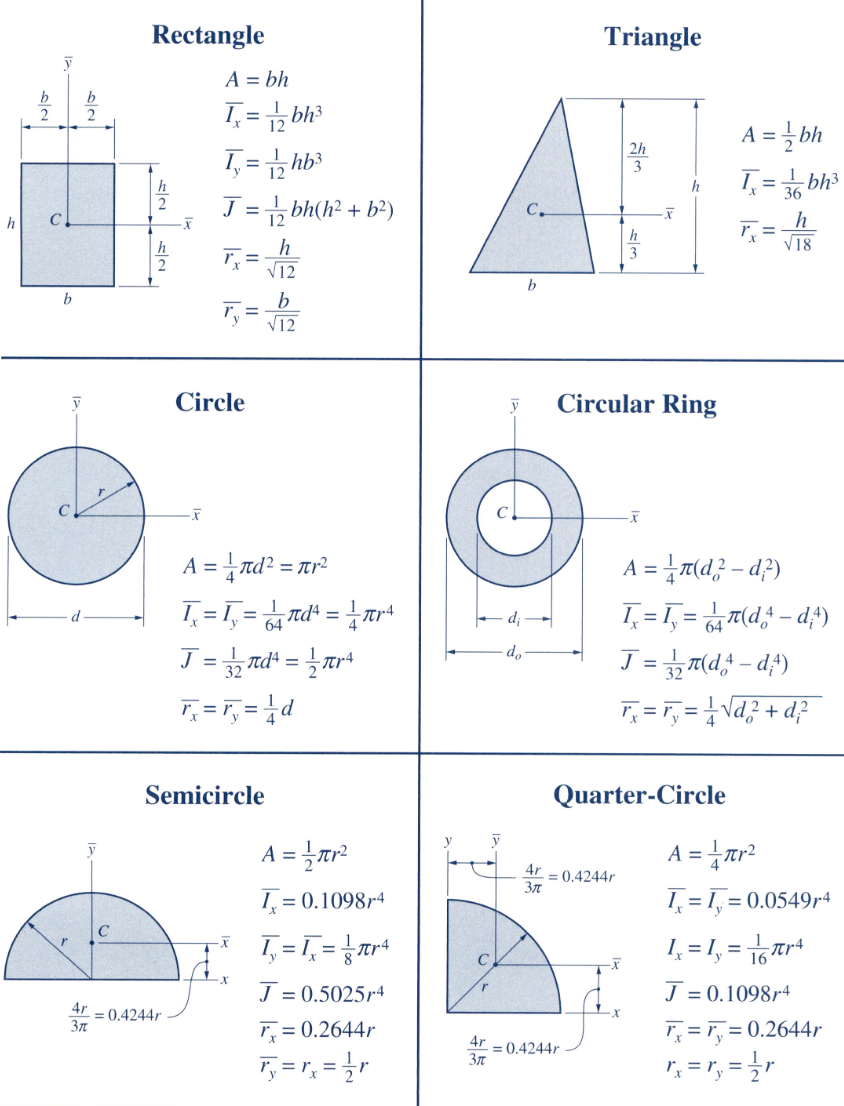
\includegraphics[width=.9\linewidth]{./images/second-moment-of-area.png}
\end{center}

\newpage

\subsection{Buoyancy force (\(F_B\))}
\label{sec:orge535c24}
\begin{itemize}
\item Buoyancy force is the resultant force acting on a submerged or partially submerged object, and it is equal to the weight of fluid displaced.
\item The direction of this force is upwards.
\end{itemize}

\[F_B = \rho g V\]

Where:
\begin{itemize}
\item \(\rho\) is the density of the fluid
\item \(g\) is the gravitational acceleration
\item \(V\) is the volume of the \textbf{fluid} displaced
\end{itemize}

\subsubsection{Density ratio}
\label{sec:org91926e0}
\[\frac{\rho_{object}}{\rho_{fluid}} = \frac{V_{submerged}}{V_{object}}\]

Where:
\begin{itemize}
\item \(\rho_{object}\) is the density of the object submerged in the fluid
\item \(\rho_{fluid}\) is the density of the fluid
\item \(V_{submerged}\) is the volume of the object submerged in the fluid
\item \(V_{object}\) is the \textbf{total} volume of the object
\end{itemize}

\newpage

\subsection{Centre of buoyancy (\(CB\))}
\label{sec:org48c0228}
\begin{itemize}
\item The centre of buoyancy is the line of action of the buoyancy force, which is vertically upwards, and it acts through the centre (centroid) of the \textbf{volume} of the fluid \textbf{displaced}.
\item For partially submerged objects, this line of action will be located at the centroid of the \textbf{volume} of the bottom half of the object, \textbf{up until the water surface}.
\item The volume of the top half of the object is \textbf{not considered}.
\item Hence, the centre of buoyancy for partially submerged objects is \textbf{not} the same as the centre of gravity of the object.
\item The centre of buoyancy for an object with \textbf{non-uniform} density is also \textbf{not} the same as the centre of gravity of the object.
\end{itemize}

\subsection{Neutral buoyancy}
\label{sec:org4358a89}
Neutral buoyancy occurs when an object's average density is equal to the density of the fluid in which it is immersed, resulting in the buoyant force balancing the force of gravity that would otherwise cause the object to sink or rise.

\[F_B = W\]

Where:
\begin{itemize}
\item \(F_B\) is the buoyancy force
\item \(W\) is the weight of the object
\end{itemize}

\subsection{Stability}
\label{sec:orgc2306ad}
An object is considered stable when it \textbf{goes back to its original position} when displaced.

\subsubsection{Fully submerged object}
\label{sec:org2c3eaab}
\begin{itemize}
\item When the centre of buoyancy is \textbf{above} the centre of gravity, the object is \textbf{stable}.
\item When the centre of buoyancy is \textbf{below} the centre of gravity, the object is \textbf{unstable}.
\end{itemize}

\subsection{Metacentre (\(M\))}
\label{sec:org8c2a5fb}
\begin{itemize}
\item Metacentre is the point of intersection of the buoyancy forces before and after rotation.
\item For a \textbf{stable} configuration, the metacentre must be \textbf{above} the centre of gravity.
\item For an \textbf{unstable} configuration, the metacentre must be \textbf{below} the centre of gravity.
\end{itemize}

\subsubsection{Determining the metacentre (\(M\))}
\label{sec:org2763e55}
\begin{enumerate}
\item Draw a vertical line passing through the centre of buoyancy
\item Tilt the object by any angle.
\item Find the centre of buoyancy for the object when it is tilted.
\item Draw a vertical line passing through the new centre of buoyancy.
\item The intersection of the two lines is the metacentre.
\end{enumerate}

\subsection{Stagnation point}
\label{sec:orge8be6b5}
The stagnation point is defined as the point where the fluid's velocity is zero.

\subsection{Bernoulli's equation along the streamline}
\label{sec:orge440ee4}
\[\frac{p_1}{\rho g} + \frac{V_1^2}{2g} + z_1 = \frac{p_2}{\rho g} + \frac{V_2^2}{2g} + z_2\]
\[p_1 + \frac{1}{2} \rho V_1^2 + \rho gz_1 = p_2 + \frac{1}{2} \rho V_2^2 + \rho gz_2\]

Where:
\begin{itemize}
\item \(p\) is the pressure of the fluid at the 2 points along the streamline
\item \(\rho\) is the density of the fluid
\item \(g\) is the gravitational acceleration
\item \(V\) is the velocity of the fluid at the 2 points along the streamline
\item \(z\) is height of the fluid above the ground at the 2 points along the streamline
\end{itemize}

\subsubsection{Assumptions}
\label{sec:org31eb54f}
\begin{itemize}
\item Inviscid flow (no viscous effect, no drag, etc.)
\item Steady flow (not changing with time)
\item Constant density (the fluid is incompressible)
\item No work or heat input
\item Along a streamline (a line tangent to velocity vectors)
\end{itemize}

\subsubsection{Flow (pressure) energy}
\label{sec:orgcc073f0}
\[\text{Pressure head} = \frac{p}{\rho g}\]

Where:
\begin{itemize}
\item \(\text{Pressure head}\) is the flow or pressure energy of the fluid
\item \(p\) is the pressure of the fluid
\item \(\rho\) is the density of the fluid
\item \(g\) is the gravitational acceleration
\end{itemize}

\subsubsection{Kinetic energy}
\label{sec:orgfa5173d}
\[\text{Velocity head} = \frac{V^2}{2g}\]

Where:
\begin{itemize}
\item \(\text{Velocity head}\) is the kinetic energy of the fluid
\item \(V\) is the velocity of the fluid
\item \(g\) is the gravitational acceleration
\end{itemize}

\subsubsection{Potential energy}
\label{sec:org90cfe0d}
\[\text{Elevation head} = z\]

Where:
\begin{itemize}
\item \(\text{Elevation head}\) is the potential energy of the fluid
\item \(z\) is the height of the fluid above the ground
\end{itemize}

\subsubsection{Static pressure}
\label{sec:orgb7de69d}
Static pressure is the actual pressure of a fluid at a point.

\[\text{Static pressure} = p\]

Where:
\begin{itemize}
\item \(p\) is the pressure of the fluid
\end{itemize}

\subsubsection{Dynamic pressure}
\label{sec:org594315a}
Dynamic pressure is the pressure due to the velocity of the fluid.

\[\text{Dynamic pressure} = \frac{\rho V^2}{2}\]

Where:
\begin{itemize}
\item \(\rho\) is the density of the fluid
\item \(V\) is the velocity of the fluid
\end{itemize}

\subsubsection{Hydrostatic pressure}
\label{sec:orgf902e53}
Hydrostatic pressure is due to the elevation of the fluid.

\[\text{Hydrostatic pressure} = \rho g z\]

Where:
\begin{itemize}
\item \(\rho\) is the density of the fluid
\item \(g\) is the gravitational acceleration
\item \(z\) is the height of the fluid above the ground
\end{itemize}

\subsubsection{Stagnation pressure}
\label{sec:orgdf917f3}
\[\text{Stagnation pressure} = p + \frac{1}{2} \rho V^2\]

Where:
\begin{itemize}
\item \(p\) is the pressure of the fluid
\item \(\rho\) is the density of the fluid
\item \(V\) is the velocity of the fluid
\end{itemize}

\newpage

\subsubsection{Total pressure}
\label{sec:orgc0ea275}
\[\text{Total pressure} = p + \frac{1}{2} \rho V^2 + \rho g z\]

Where:
\begin{itemize}
\item \(p\) is the pressure of the fluid
\item \(\rho\) is the density of the fluid
\item \(V\) is the velocity of the fluid
\item \(g\) is the gravitational acceleration
\item \(z\) is the height of the fluid above the ground
\end{itemize}

\subsection{Bernoulli's equation across the streamline}
\label{sec:orgbc40598}
\[\frac{\partial \left(p + \rho g z \right)}{\partial n} = - \frac{\rho V^2}{R}\]

Where:
\begin{itemize}
\item \(p\) is the pressure of the fluid
\item \(\rho\) is the density of the fluid
\item \(g\) is the gravitational acceleration
\item \(z\) is the height of the fluid
\item \(\partial n\) is the partial derivative with respect to the axis across the streamline
\item \(V\) is the velocity of the fluid
\item \(R\) is the radius of the circular arc of the rotating streamline. \(R\) is infinity when the streamline is straight.
\end{itemize}

\subsection{Mass continuity equation}
\label{sec:orgd5372ae}
\[A_1 V_1 = A_2 V_2\]

Where:
\begin{itemize}
\item \(A\) is the cross-sectional area of the fluid at each point. This cross-sectional area must be perpendicular to the velocity of the fluid.
\item \(V\) is the velocity of the fluid at each point
\end{itemize}

\subsection{Large tank assumption}
\label{sec:orgdb2c965}
The velocity of the fluid moving down from the top of the tank can be taken to be zero if the tank is at least \textbf{4 times} the size of the outlet.

\subsection{Vapour pressure (\(p_v\))}
\label{sec:org282775a}
\begin{itemize}
\item Vapour pressure is the pressure of the vapour bubbles formed in a liquid at \textbf{room temperature}.
\item For \(H_{2}O\) at \(\qty{15}{\degreeCelsius}\), the vapour pressure \(p_v\) is \(\qty{1700}{Pa}\).
\end{itemize}

\subsection{Cavitation}
\label{sec:orgff9a787}
When the pressure drops to the vapour pressure, vapour bubbles are formed. Basically, cavitation occurs at saturation pressure (\(P_{sat}\)).

\subsubsection{Negative effects of cavitation}
\label{sec:org9e3b69e}
\begin{enumerate}
\item The vapour bubbles may burst to cause corrosion and subsequent structural failure on pump blades.
\item The efficiency of a pump may be reduced as each pump is designed to deliver liquids (not bubbles) only.
\end{enumerate}

\subsection{Velocity field}
\label{sec:orgdccb390}
\[\boldsymbol{V} = u(x, y, z, t) \boldsymbol{i} + v(x, y, z, t) \boldsymbol{j} + v(x, y, z, t) \boldsymbol{k}\]

Where:
\begin{itemize}
\item \(\boldsymbol{V}\) is the velocity field
\item \(u, v, w\) are the \(x, y, z\) components of the velocity vector respectively
\end{itemize}

\subsubsection{Magnitude}
\label{sec:orgc5e1aa6}
\[\left| \boldsymbol{V} \right| = \sqrt{u^2 + v^2 + w^2}\]

Where:
\begin{itemize}
\item \(\left| \boldsymbol{V} \right|\) is the speed of the fluid
\item \(u, v, w\) are the \(x, y, z\) components of the velocity vector respectively
\end{itemize}

\subsection{Flow analysis methods}
\label{sec:org1f79d46}

\subsubsection{Lagrangian method}
\label{sec:orgc19cb07}
The Lagrangian method follows the individual fluid particles.

\subsubsection{Eulerian method}
\label{sec:orgc0a982e}
\begin{itemize}
\item The Eulerian method studies the flow that passes through a fixed space.
\item Usually, the Eulerian method is used in fluid mechanics.
\end{itemize}

\subsection{Streamlines}
\label{sec:org3c41857}
A streamline is the curve formed by velocity vectors of each fluid particle at a certain time.

\subsection{Streak lines}
\label{sec:org41654f9}
A streak line is a line formed by fluid particles that pass a fixed point in the stream.

\subsection{Path lines}
\label{sec:orgc3c15d1}
A path line is the path of one particular fluid particle.

\subsection{Newton's second law}
\label{sec:org77a534e}
The rate of change of momentum of a system is equal to the sum of all the forces acting on the system. Essentially:
\[\frac{dp}{dt} = \frac{\Delta m \Delta v}{\Delta t} = \sum F = F_{net}\]

Where:
\begin{itemize}
\item \(\frac{dp}{dt}\) is the rate of change of momentum with respect to time
\item \(\Delta m\) is the change in mass
\item \(\Delta v\) is the change in velocity
\item \(\Delta t\) is the change in time
\item \(\sum F\) and \(F_{net}\) is the net force acting on an object
\end{itemize}

\subsection{Reynold's transport theorem (RTT)}
\label{sec:org8304310}
\[\frac{dB_{sys}}{dt} = \frac{\partial}{\partial t} \int_{CV} \rho b \, dV + \int_{CS} \rho b \boldsymbol{V} \cdot \boldsymbol{n} \, dA\]

Where:
\begin{itemize}
\item \(\frac{dB_{sys}}{dt}\) is the rate of change of \(B\) of a system with respect to time
\item \(\frac{\partial}{\partial t} \int_{CV} \rho b \, dV\) is the rate of change of \(B\) within the control volume with respect to time
\item \(\int_{CS} \rho b \boldsymbol{V} \cdot \boldsymbol{n} \, dA\) is the net flow rate of \(B\) through the \textbf{entire control surface}
\item \(B\) represents any of the fluid parameters, \(B = bm\), which is an extensive property
\item \(b\) represent the amount of that parameter per unit mass, which is an intensive property
\item \(\rho\) is the density of the fluid
\item \(dV\) is the infinitesimal volume of the system
\item \(\boldsymbol{V}\) is the \textbf{velocity vector} of the fluid particle
\item \(\boldsymbol{n}\) is the \textbf{outward normal unit vector} of the control surface
\end{itemize}

\subsubsection{B for the system and control volume}
\label{sec:org1cc861b}
\[B_{sys} = \int_{sys} \rho b \, dV\]
\[B_{CV} = \int_{CV} \rho b \, dV\]

Where:
\begin{itemize}
\item \(B\) represents any of the fluid parameters, \(B = bm\), which is an extensive property
\item \(b\) represent the amount of that parameter per unit mass, which is an intensive property
\item \(\rho\) is the density of the fluid
\item \(dV\) is the infinitesimal volume of the system
\end{itemize}

\subsubsection{With steady flow}
\label{sec:orgffa4975}
\[\frac{\partial}{\partial t} = 0\]
\[\frac{dB_{sys}}{dt} = \int_{CS} \rho b \boldsymbol{V} \cdot \boldsymbol{n} \, dA\]

Where:
\begin{itemize}
\item \(\frac{dB_{sys}}{dt}\) is the rate of change of \(B\) of a system with respect to time
\item \(\int_{CS} \rho b \boldsymbol{V} \cdot \boldsymbol{n} \, dA\) is the net flow rate of \(B\) through the \textbf{entire control surface}
\item \(B\) represents any of the fluid parameters, \(B = bm\), which is an extensive property
\item \(b\) represent the amount of that parameter per unit mass, which is an intensive property
\item \(\rho\) is the density of the fluid
\item \(\boldsymbol{V}\) is the \textbf{velocity vector} of the fluid particle
\item \(\boldsymbol{n}\) is the \textbf{outward normal unit vector} of the control surface
\end{itemize}

\newpage

\subsubsection{With control volume moving at constant speed}
\label{sec:org04d51c6}
\begin{itemize}
\item If the control volume is moving at velocity \(\boldsymbol{V_{CV}}\), an observer fixed to the control volume will see a relative velocity \(\boldsymbol{W}\) of the fluid crossing the control volume.
\item Relationship between absolute velocity \(\boldsymbol{V}\), velocity of the control volume \(V_{CV}\) and relative velocity \(\boldsymbol{W}\) is:
\[\boldsymbol{V} = \boldsymbol{W} + \boldsymbol{V_{CV}}\]
\end{itemize}

\[\frac{dB_{sys}}{dt} = \frac{\partial}{\partial t} \int_{CV} \rho b \, dV + \int_{CS} \rho b \boldsymbol{W} \cdot \boldsymbol{n} \, dA\]

Where:
\begin{itemize}
\item \(\frac{dB_{sys}}{dt}\) is the rate of change of \(B\) of a system with respect to time
\item \(\frac{\partial}{\partial t} \int_{CV} \rho b \, dV\) is the rate of change of \(B\) within the control volume with respect to time
\item \(\int_{CS} \rho b \boldsymbol{W} \cdot \boldsymbol{n} \, dA\) is the net flow rate of \(B\) through the \textbf{entire control surface}
\item \(B\) represents any of the fluid parameters, \(B = bm\), which is an extensive property
\item \(b\) represent the amount of that parameter per unit mass, which is an intensive property
\item \(\rho\) is the density of the fluid
\item \(dV\) is the infinitesimal volume of the system
\item \(\boldsymbol{W}\) is the \textbf{relative velocity vector} of the fluid particle
\item \(\boldsymbol{n}\) is the \textbf{outward normal unit vector} of the control surface
\end{itemize}

\newpage

\subsection{Continuity equation}
\label{sec:org45094ac}
When \(\frac{dm_{sys}}{dt} = 0\),
\[B = m\]
\[b = 1\]

\[\therefore \frac{dm_{sys}}{dt} = 0 = \frac{\partial}{\partial t} \int_{CV} \rho \, dV + \int_{CS} \rho \boldsymbol{V} \cdot \boldsymbol{n} \, dA\]

Which results in the continuity equation:
\[\frac{\partial}{\partial t} \int_{CV} \rho \, dV + \int_{CS} \rho \boldsymbol{V} \cdot \boldsymbol{n} \, dA = 0\]

Where:
\begin{itemize}
\item \(\frac{dm_{sys}}{dt}\) is the rate of change of mass of a system with respect to time
\item \(\frac{\partial}{\partial t} \int_{CV} \rho \, dV\) is the rate of change of the mass content of the control volume with respect to time.
\item \(\int_{CS} \rho \boldsymbol{V} \cdot \boldsymbol{n} \, dA\) is the net mass flow rate through the \textbf{entire control surface}
\item \(B\) represents any of the fluid parameters, \(B = bm\), which is an extensive property
\item \(b\) represent the amount of that parameter per unit mass, which is an intensive property
\item \(\rho\) is the density of the fluid
\item \(dV\) is the infinitesimal volume of the system
\item \(\boldsymbol{V}\) is the \textbf{velocity vector} of the fluid particle
\item \(\boldsymbol{n}\) is the \textbf{outward normal unit vector} of the control surface
\end{itemize}

\newpage

\subsubsection{With steady flow}
\label{sec:org9c68d3d}
When the flow is steady,
\[\frac{\partial}{\partial t} = \int_{CV} \rho \, dV = 0\]

Hence:
\[\int_{CS} \rho \boldsymbol{V} \cdot \boldsymbol{n} \, dA = \sum \dot{m}_{out} - \sum \dot{m}_{in} = 0\]

Where:
\begin{itemize}
\item \(\int_{CS} \rho \boldsymbol{V} \cdot \boldsymbol{n} \, dA\) is the net mass flow rate through the \textbf{entire control surface}
\item \(\dot{m}_{out}\) is the mass flow rate out of the system
\item \(\dot{m}_{in}\) is the mass flow rate into the system
\end{itemize}

\subsubsection{With steady flow and incompressible fluid}
\label{sec:org951767c}
\[\int_{CS} \rho \boldsymbol{V} \cdot \boldsymbol{n} \, dA = \sum Q_{out} - \sum Q_{in} = 0\]

Where:
\begin{itemize}
\item \(\int_{CS} \rho \boldsymbol{V} \cdot \boldsymbol{n} \, dA\) is the net mass flow rate through the \textbf{entire control surface}
\item \(Q_{out}\) is the volume flow rate out of the system
\item \(Q_{in}\) is the volume flow rate into the system
\end{itemize}

\subsubsection{With uniformly distributed flow over the control surface opening}
\label{sec:orge142f61}
\[\dot{m} = \rho A V\]

Where:
\begin{itemize}
\item \(\dot{m}\) is the net mass flow rate through the \textbf{entire control surface}
\item \(\rho\) is the density of the fluid
\item \(A\) is the area of the control surface
\item \(V\) is the velocity component \textbf{perpendicular} to the control surface
\end{itemize}

\subsubsection{With uniformly distributed flow over the control surface opening but non-uniformly distributed velocity}
\label{sec:org2dde1df}
\[\dot{m} = \rho A \overline{V}\]
\[\overline{V} = \frac{\int_A \rho \boldsymbol{V} \cdot \boldsymbol{n} \, dA}{\rho A}\]

Where:
\begin{itemize}
\item \(\dot{m}\) is the net mass flow rate through the \textbf{entire control surface}
\item \(\rho\) is the density of the fluid
\item \(A\) is the area of the control surface
\item \(\overline{V}\) is the \textbf{average} velocity component \textbf{perpendicular} to the control surface
\end{itemize}

\subsection{Mass flow rate}
\label{sec:org591b98e}
\[\dot{m} = \int_A \rho \boldsymbol{V} \cdot \boldsymbol{n} \, dA\]

Where:
\begin{itemize}
\item \(\dot{m}\) is the mass flow rate through a control surface of area \(A\)
\item \(A\) is the area of the control surface
\item \(\rho\) is the density of the fluid
\item \(\boldsymbol{V}\) is the \textbf{velocity vector} of the fluid particle
\item \(\boldsymbol{n}\) is the \textbf{outward normal unit vector} of the control surface
\end{itemize}

\subsection{Volume flow rate}
\label{sec:orgc2857c3}
\[Q = \int_A \boldsymbol{V} \cdot \boldsymbol{n} \, dA\]

Where:
\begin{itemize}
\item \(Q\) is the volume flow rate through a control surface of area \(A\)
\item \(A\) is the area of the control surface
\item \(\boldsymbol{V}\) is the \textbf{velocity vector} of the fluid particle
\item \(\boldsymbol{n}\) is the \textbf{outward normal unit vector} of the control surface
\end{itemize}

\newpage

\section{Types of systems}
\label{sec:orgd65bb54}
\begin{center}
\begin{tabular}{l|l|l}
Type of system & Mass flow & Heat\\[0pt]
\hline
Open system & Yes & Yes\\[0pt]
Closed system & No & Yes\\[0pt]
Isolated system & No & No\\[0pt]
\end{tabular}
\end{center}


\section{Boiling process}
\label{sec:orga09bf44}
A closed system, comprising a pure substance, heated at constant pressure passes through several phases:
\begin{itemize}
\item Subcooled or compressed liquid (the liquid does not vaporise except for normal evaporation)
\item Saturated liquid (the liquid is about the vaporise)
\item Saturated liquid-vapour mixture
\item Saturated vapour (the vapour is about to condense)
\item Superheated vapour (the vapour is heated beyond the condensation point and hence does not condense)
\end{itemize}


\section{States}
\label{sec:orgcf2254a}
\begin{center}
\begin{tabular}{l|l}
State & Requirements\\[0pt]
\hline
Supercritical & T > T\textsubscript{critical} \& P > P\textsubscript{critical}\\[0pt]
Compressed liquid & P < P\textsubscript{critical} \& T < T\textsubscript{sat} or P > P\textsubscript{critical} \& T < T\textsubscript{critical}\\[0pt]
Saturated liquid-vapour mixture & P < P\textsubscript{critical} \& T = T\textsubscript{sat}\\[0pt]
Superheated vapour & P < P\textsubscript{critical} \& T > T\textsubscript{sat}\\[0pt]
\end{tabular}
\end{center}

\newpage

\section{Steam table}
\label{sec:org761e7f3}

\subsection{Table A4}
\label{sec:orgad09eb5}
For calculating the saturation properties at a given \textbf{temperature}.

\subsection{Table A5}
\label{sec:orgcf85d79}
For calculating the saturated properties at a given \textbf{pressure}.

\subsection{Table A6}
\label{sec:org15eabfa}
For calculating the superheated properties. Two independent intrinsic properties are required, for example:
\begin{itemize}
\item Pressure and temperature
\item Pressure and volume
\item Temperature and volume
\item Pressure and internal energy
\item Temperature and internal energy
\item Volume and internal energy
\end{itemize}

\subsection{Table A7}
\label{sec:org872dc63}
For calculating the compressed liquid properties.

\subsection{R-134a (a refrigerant)}
\label{sec:orgc1c57ce}
Includes additional tables A11 - A13

\subsubsection{Table A11}
\label{sec:orgaef8991}
For calculating saturated properties.

\subsubsection{Table A12}
\label{sec:org834b43c}
For calculating saturated properties as well.

\subsubsection{Table A13}
\label{sec:org104ee6c}
For calculating superheated properties.

\subsection{Saturated liquid-vapour tables}
\label{sec:org37174ef}
\begin{itemize}
\item \textbf{Temperature or pressure} given as the first column
\item \textbf{Saturated liquid} (\(f\)), \textbf{saturated vapour} (\(g\)) values and evaporation (\(fg\)) values given for other properties.
\begin{itemize}
\item "\(v\)" is the specific \textbf{volume}
\item "\(u\)" is the specific \textbf{internal energy}
\item "\(h\)" is the specific \textbf{enthalpy}
\item "\(s\)" is the specific \textbf{entropy}
\end{itemize}
\end{itemize}

\subsection{Superheated vapour tables}
\label{sec:orgbccec85}
Use the superheated vapour tables if:
\begin{itemize}
\item \(P < P_{sat}\) for a given \(T\)
\item \(T > T_{sat}\) for a given \(P\)
\item \(v > v_g, u > u_g, h > h_g\) for given \(P\) and \(T\)
\end{itemize}

\subsection{Compressed liquid tables}
\label{sec:org7458488}
Use the compressed liquid tables if:
\begin{itemize}
\item \(T < T_{sat}\) for a given \(P\)
\item \(P > P_{sat}\) for a given \(T\)
\end{itemize}

\subsubsection{Other properties}
\label{sec:org8b193f9}
\(v \approx v_f, u \approx u_f, h \approx h_f\) for given \(P\) and \(T\)
\begin{itemize}
\item These properties are more dependent on temperature \(T\) as compared to pressure \(P\)
\item For a better estimate of \(h\):
\[h \approx h_{f@T} + v_{f@T} (P - P_{sat})\]
\end{itemize}


\section{Generalised compressibility chart}
\label{sec:orge69aec3}
\begin{itemize}
\item Principle of corresponding states: gases behave similarly when normalised with respect to their critical pressure and temperature.
\item The normalised variables are called \textbf{reduced pressure (\(P_R\))} and \textbf{reduced temperature (\(T_R\))}.
\item The pressure or temperature of a gas is high or low relative to its critical temperature or pressure
\item The lines that look like a checkmark or a tick on the generalised compressibility chart are the reduced temperature (\(T_R\)) lines.
\item The lines that start from the bottom and then get higher over time are the pseudo-reduced specific volume (\(v_R\)) lines.
\end{itemize}

\newpage

\section{Thermodynamic processes}
\label{sec:org5c30f30}
The prefix \emph{iso-} is used to define a process with a constant property.

\subsection{Isothermal process}
\label{sec:org8be431b}
\begin{itemize}
\item A process during which the temperature \(T\) remains constant.
\item An isothermal system has equivalent temperatures in and out of the system under one state.
\end{itemize}

\subsubsection{Work done}
\label{sec:org83287ce}
\[W_b = \int_1^2 P \, dV = \int_1^2 \frac{C}{V} \, dV = C \ln \left(\frac{V_2}{V_1} \right) = C \ln \left(\frac{P_1}{P_2} \right)\]

Where:
\begin{itemize}
\item \(W_B\) is the work done
\item \(P\) is the pressure on the system
\item \(dV\) is the infinitesimal change in volume of the system
\item \(V_2\) is the \textbf{final} volume of the system
\item \(V_1\) is the \textbf{initial} volume of the system
\item \(P_1\) is the \textbf{initial} pressure of the system
\item \(P_2\) is the \textbf{final} pressure of the system
\item \(C\) is a constant given by:

\[C = PV = m R_m T = nRT\]

Where:
\begin{itemize}
\item \(P\) is the pressure on the system
\item \(V\) is the volume on the system
\item \(m\) is the mass of the gas
\item \(R_m\) is the gas constant in terms of mass
\item \(T\) is the temperature of the gas
\item \(n\) is the number of moles of the gas
\item \(R\) is the molar gas constant
\end{itemize}
\end{itemize}

\subsection{Isobaric process}
\label{sec:orgc1bbf07}
\begin{itemize}
\item A process during which the pressure \(P\) remains constant.
\item Some examples include a piston-cylinder setup where the \textbf{piston is free to move}.
\end{itemize}

\subsubsection{Work done}
\label{sec:org981624c}
The work done \(W\) is equal to the pressure \(P\) multiplied by the change in volume \(V_2 - V_1\). I.e:

\[W_b = P \left(V_2 - V_1 \right)\]

Where:
\begin{itemize}
\item \(W_b\) is the work done
\item \(P\) is the pressure of the system
\item \(V_2\) is the \textbf{final} volume of the system
\item \(V_1\) is the \textbf{initial} volume of the system
\end{itemize}

\subsection{Isochoric (isometric) process}
\label{sec:org2512847}
\begin{itemize}
\item A process during which the specific volume \(v\) remains constant.
\item The work done \(W_b\) of such a process is 0.
\end{itemize}

\subsection{Reversible and adiabatic process (isentropic process)}
\label{sec:org30c51c8}
\begin{itemize}
\item A reversible process with \textbf{no heat transfer}.
\item Some examples include a well insulated system, and a system at the same temperature as its surroundings.
\item An adiabatic process is \textbf{not} an isothermal process.
\item A system with no heat transfer can have its temperature changed by other means, like work done.
\end{itemize}

\subsection{Polytropic Process}
\label{sec:org82759c2}
A process such that pressure and volume of a gas is given by:
\[PV^n = C \text{ where } n \ne 1\]

Where:
\begin{itemize}
\item \(P\) is the pressure on the system
\item \(V\) is the volume of the system
\item \(n\) is the polytropic index
\end{itemize}

When \(n = k = \frac{c_p}{c_v}\), the polytropic process becomes an isentropic or adiabatic process.
\begin{itemize}
\item \(k\) is the specific heat ratio
\item \(c_p\) is the specific heat capacity at constant pressure
\item \(c_v\) is the specific heat capacity at constant volume
\end{itemize}

\newpage

\subsubsection{Work done}
\label{sec:org4a0b76d}
\[W_b = \frac{P_2 V_2 - P_1 V_1}{1 - n}\]

Where:
\begin{itemize}
\item \(W_b\) is the work done
\item \(P_2\) is the \textbf{final} pressure on the system
\item \(V_2\) is the \textbf{final} volume of the system
\item \(P_1\) is the \textbf{initial} pressure on the system
\item \(V_1\) is the \textbf{initial} volume on the system
\item \(n\) is the power that the \(V\) term is raised to, or the polytropic index
\end{itemize}

If the gas behaves like an \textbf{ideal gas}, then the work done will be:
\[W_b = \frac{m R_m (T_2 - T_1)}{1 - n}\]

Where:
\begin{itemize}
\item \(m\) is the mass of the gas
\item \(R_m\) is the gas constant in terms of mass
\item \(T_2\) is the \textbf{final} temperature of the system
\item \(T_1\) is the initial temperature of the system
\item \(n\) is the power that the \(V\) term is raised to, or the polytropic index
\end{itemize}

\subsection{Isenthalpic process (constant enthalpy process)}
\label{sec:org9ebc6d0}
A process in which there is no change in enthalpy, i.e. \(\Delta H = H_2 - H_1 = 0\).

\newpage

\section{Incompressible fluids}
\label{sec:org541873a}
\begin{itemize}
\item Applies to solids and most liquids
\item Specific volume \(v\) is assumed to be \textbf{constant}
\item Specific internal energy \(u\) is a function of temperature \(T\) only, \(u = u(T)\)
\item Specific heat at constant pressure is equal to the specific heat at constant volume \(c_p = c_v\)
\item Hence, incompressible fluids only have specific heat \(c\), as there is no difference between \(c_p\) and \(c_v\).
\end{itemize}

\subsection{Internal energy change}
\label{sec:org4260041}
\[\Delta u = u_2 - u_1 \cong c_{avg} \left(T_2 - T_1 \right)\]

Where:
\begin{itemize}
\item \(\Delta u\) is the change in internal energy
\item \(u_2\) is the \textbf{final} specific internal energy
\item \(u_1\) is the \textbf{initial} specific internal energy
\item \(c_{avg}\) is the specific heat capacity of the fluid calculated at an average temperature
\item \(T_2\) is the \textbf{final} temperature
\item \(T_1\) is the \textbf{initial} temperature
\end{itemize}

\newpage

\subsection{Enthalpy change}
\label{sec:orga9d235f}
\[\Delta h = h_2 - h_1 \cong c_{avg} \left(T_2 - T_1 \right) + v \left(P_2 - P_1 \right)\]

Where:
\begin{itemize}
\item \(\Delta h\) is the change in enthalpy
\item \(h_2\) is the \textbf{final} specific enthalpy
\item \(h_1\) is the \textbf{initial} specific enthalpy
\item \(c_{avg}\) is the specific heat capacity of the fluid calculated at an average temperature
\item \(T_2\) is the \textbf{final} temperature
\item \(T_1\) is the \textbf{initial} temperature
\item \(v\) is the specific volume of the fluid
\item \(P_2\) is the \textbf{final} pressure
\item \(P_1\) is the \textbf{initial} pressure
\end{itemize}

\newpage

\section{Energy balance for closed systems}
\label{sec:org5b9a66f}
\[\Delta E_{\text{system}} = E_2 - E_1\]

Where:
\begin{itemize}
\item \(\Delta E_{\text{system}}\) is the change in energy of the system
\item \(E_2\) is the \textbf{final} energy of the system
\item \(E_1\) is the \textbf{initial} energy of the system
\end{itemize}

For closed systems, the energy transfer is only due to heat or work
\[E_{in} - E_{out} = (Q_{in} - Q_{out}) + (W_{in} - W_{out})\]

Where:
\begin{itemize}
\item \(E_{in}\) is the energy input into the system
\item \(E_{out}\) is the energy leaving the system
\item \(Q_{in}\) is the heat input into the system
\item \(Q_{out}\) is the heat leaving the system
\item \(W_{in}\) is the work done on the system
\item \(W_{out}\) is the work done by the system
\end{itemize}

\subsection{Sign conventions}
\label{sec:org58e8cb3}
\begin{itemize}
\item Heat transferred \textbf{to} the system is positive.
\[Q = Q_{in} - Q_{out}\]

\item Work produced \textbf{by} the system is positive.
\[W = W_{out} - W_{in}\]
\end{itemize}

Hence:
\[\Delta E_{\text{system}} = E_{in} - E_{out} = Q - W\]

Where:
\begin{itemize}
\item \(E_{in}\) is the energy input into the system
\item \(E_{out}\) is the energy leaving the system
\item \(Q\) is the heat \textbf{transferred to} the system
\item \(W\) is the work done \textbf{by} the system
\end{itemize}

\subsection{First law of thermodynamics}
\label{sec:orge88c768}
\[E_2 - E_1 = (Q_{in} - Q_{out}) + (W_{in} - W_{out})\]
\[Q - W = E_2 - E_1\]

Where:
\begin{itemize}
\item \(E_2\) is the \textbf{final} energy of the system
\item \(E_1\) is the \textbf{initial} energy of the system
\item \(Q_{in}\) is the heat input into the system
\item \(Q_{out}\) is the heat leaving the system
\item \(W_{in}\) is the work done on the system
\item \(W_{out}\) is the work done by the system
\item \(Q\) is the \textbf{heat transferred} to the system
\item \(W\) is the work done \textbf{by} the system
\end{itemize}

\subsubsection{Stationary system}
\label{sec:org1aead1a}
\[Q - W = \Delta U = U_2 - U_1\]

Where:
\begin{itemize}
\item \(Q\) is the \textbf{heat transferred} to the system
\item \(W\) is the work done \textbf{by} the system
\item \(\Delta U\) is the change in internal energy of the system
\item \(U_2\) is the \textbf{final} internal energy of the system
\item \(U_1\) is the \textbf{initial} internal energy of the system
\end{itemize}


\section{Steady flow engineering devices}
\label{sec:org4fa2dd0}
Many engineering devices operate under the same conditions over long periods of time, such as in power plants and industrial processes. These include:
\begin{itemize}
\item Nozzles and diffusers
\item Turbines and compressors
\item Throttling valves
\item Mixing chambers
\item Heat exchangers
\item Pipe and duct flow
\end{itemize}

\subsection{Nozzle}
\label{sec:org9ee2402}
A nozzle is a device to increase the velocity of a fluid.
\begin{itemize}
\item It has a single inlet and exit.
\item There is no work done, i.e. \(\dot{W} = 0\).
\item The change in potential energy is assumed to be zero, i.e. \(\Delta \text{pe} = 0\).
\item The change in kinetic energy is usually small compared to the change in enthalpy and can be assumed to be zero, i.e. \(\text{ke} = 0\).
\end{itemize}

\subsection{Diffuser}
\label{sec:orgdf4f05f}
A diffuser is a device for reducing the velocity and increasing the static pressure of a fluid passing through a system.
\begin{itemize}
\item It has a single inlet and exit.
\item The velocity of the fluid at the outlet can be assumed to be \(0\).
\item There is no work done, i.e. \(\dot{W} = 0\).
\item The change in potential energy is assumed to be zero, i.e. \(\Delta \text{pe} = 0\).
\item The change in kinetic energy is usually small compared to the change in enthalpy and can be assumed to be zero, i.e. \(\text{ke} = 0\).
\end{itemize}

\subsection{Turbine}
\label{sec:orgf98706b}
A turbine is a device to produce work from the flow of a gas through a set of blades attached to a freely rotating shaft.
\begin{itemize}
\item It is used in power generation and jet engines.
\item It has a single inlet and exit.
\item Work is produced by the turbine, which means the work done is positive, i.e. \(\dot{W} > 0\)
\item The change in potential energy is assumed to be zero, i.e. \(\Delta \text{pe} = 0\).
\item The change in kinetic energy is usually small compared to the change in enthalpy and can be assumed to be zero, i.e. \(\text{ke} = 0\).
\item Heat losses are assumed to be small, i.e. \(\dot{Q} = 0\).
\item If there is no cooling or heat losses, i.e. an adiabatic process where \(\dot{Q} = 0\):
\[\dot{W} = \dot{m} \left(h_i - h_e \right)\]

Where:
\begin{itemize}
\item \(\dot{W}\) is the power output of the turbine
\item \(\dot{m}\) is the mass flow rate through the turbine
\item \(h_i\) is the \textbf{initial} enthalpy of the fluid
\item \(h_e\) is the \textbf{final} enthalpy of the fluid
\end{itemize}
\end{itemize}

\newpage

\subsection{Compressors, pumps and fans}
\label{sec:org8a5926e}
Compressors, pumps and fans are devices used to increase pressure of a fluid and requires work input.
\begin{itemize}
\item Compressors compresses gas to high pressures.
\item Pumps handle liquids.
\item Fans move air while increasing the pressure slightly.
\item These devices have a single inlet and exit.
\item Work is needed for these devices, which means the work done is negative, i.e. \(\dot{W} < 0\).
\item The change in potential energy is assumed to be zero, i.e. \(\Delta \text{pe} = 0\).
\item The change in kinetic energy is usually small compared to the change in enthalpy and can be assumed to be zero, i.e. \(\text{ke} = 0\).
\item Compressors often require some cooling that means the heat transferred is negative, i.e. \(\dot{Q} = \dot{m} q_{out} < 0\).
\item If there is no cooling or heat losses, i.e. an adiabatic process where \(\dot{Q} = 0\):
\[\dot{W} = \dot{m} \left(h_e - h_i \right)\]

Where:
\begin{itemize}
\item \(\dot{W}\) is the power output of the turbine
\item \(\dot{m}\) is the mass flow rate through the turbine
\item \(h_e\) is the \textbf{final} enthalpy of the fluid
\item \(h_i\) is the \textbf{initial} enthalpy of the fluid
\end{itemize}
\end{itemize}

\newpage

\subsection{Throttling valves}
\label{sec:org777d8ff}
Throttling valves are flow-restricting devices having significant pressure drop with no work done and minimal heat transfer to the surroundings.
\begin{itemize}
\item There is no work done, i.e. \(\dot{W} = 0\).
\item Heat transfer is assumed to be negligible, i.e. \(\dot{Q} = 0\).
\item The change in potential energy is assumed to be zero, i.e. \(\Delta \text{pe} = 0\).
\item The change in kinetic energy is usually small compared to the change in enthalpy and can be assumed to be zero, i.e. \(\text{ke} = 0\).
\item It usually results in a \textbf{temperature drop} if there is phase change, which is the case in refrigeration and air-conditioning applications.
\item It is a constant enthalpy process, which means \(h_i = h_e\).
\item In the case of an ideal gas, the process is isothermal.
\item The enthalpy of the fluid remains constant, but the internal energy and flow energy may be converted into one another:
\[u_1 + P_1 v_1 = u_2 + P_2 v_2\]

Where:
\begin{itemize}
\item \(u_1\) is the initial internal energy
\item \(P_1\) is the initial pressure
\item \(v_1\) is the initial \textbf{specific} volume
\item \(u_2\) is the final internal energy
\item \(P_2\) is the final pressure
\item \(v_2\) is the final \textbf{specific} volume
\end{itemize}
\end{itemize}

\newpage

\subsection{Mixing chambers}
\label{sec:orgcbc1f6a}
Mixing chambers are devices that combine two or more streams at different conditions, to produce a single mixed stream.
\begin{itemize}
\item The mass balance is \(\sum \dot{m}_i = \dot{m}_e\).
\item The heat transferred and work done is assumed to be zero, i.e. \(\dot{Q} = 0\) and \(\dot{W} = 0\).
\item The change in potential energy and kinetic energy is also assumed to be zero, i.e. \(\Delta \text{pe} = 0\) and \(\Delta \text{ke} = 0\).
\item The energy balance is:
\[\sum \dot{m}_i h_i = \dot{m}_e h_e\].
\end{itemize}

\subsection{Heat exchangers}
\label{sec:orgbd7e1b1}
Heat exchangers are devices that transfer energy between moving fluid streams at different temperatures.
\begin{itemize}
\item The change in potential energy and kinetic energy is also assumed to be zero, i.e. \(\Delta \text{pe} = 0\) and \(\Delta \text{ke} = 0\).
\item The work done is assumed to be zero, i.e. \(\dot{W} = 0\).
\end{itemize}

\subsubsection{Whole heat exchanger as control volume}
\label{sec:org3a8fef2}
\begin{itemize}
\item The heat transferred is zero, i.e. \(\dot{Q} = 0\).
\item The energy balance is:
\[\sum \dot{m}_i h_i = \sum \dot{m}_e h_e\]
\end{itemize}

\subsubsection{Fluid inside the heat exchanger as control volume}
\label{sec:org9154400}
\begin{itemize}
\item There is one inlet and one outlet.
\item The energy balance is:
\[\dot{Q}_{fluid} = \dot{m}_{fluid} \left(h_{e_{fluid}} - h_{i_{fluid}} \right)\]
\end{itemize}


\section{Pressure variation in a fluid}
\label{sec:org0fa6098}
\[\frac{\partial p}{\partial x} = - \rho a_x\]
\[\frac{\partial p}{\partial y} = - \rho a_y\]
\[\frac{\partial p}{\partial z} = - \rho (g + a_z)\]

Where:
\begin{itemize}
\item \(\frac{\partial p}{\partial x}, \frac{\partial p}{\partial y}, \frac{\partial p}{\partial z}\) is the partial derivative of pressure with respect to the \(x, y\) and \(z\) directions respectively
\item \(\rho\) is the density of the fluid
\item \(a_x, a_y, a_y\) is the acceleration of the fluid in the \(x, y\) and \(z\) direction respectively
\item \(g\) is the gravitational acceleration
\end{itemize}

\subsection{For the case of no acceleration}
\label{sec:org21827c2}
\[a_x = a_y = a_z = 0\]

The above equations simplify to:
\begin{align*}
\frac{dp}{dz} &= - \rho g \\
\int_{p_1}^{p_2} \, dp &= - \int_{z_1}^{z_2} \rho g \, dz \\
p_2 - p_1 &= - \rho g (z_2 - z_1) \\
p_2 - p_1 &= \rho g (z_1 - z_2) \\
\end{align*}

Where:
\begin{itemize}
\item \(p_2\) is the final pressure of the fluid
\item \(p_1\) is the initial pressure of the fluid
\item \(\rho\) is the density of the fluid
\item \(g\) is the gravitational acceleration
\item \(z_2\) is the final height of the fluid
\item \(z_1\) is the initial height of the fluid
\end{itemize}

\subsubsection{In terms of depth \(h\)}
\label{sec:org8a6fecb}
Substituting \(p_1 = p_{atm}\), \(h = - z_2\), and \(z_1 = 0\) where \(h\) is the depth of the fluid,

\begin{align*}
p_2 - p_{atm} &= \rho g (0 + h) \\
p_2 - p_{atm} &= \rho g h
\end{align*}

Where:
\begin{itemize}
\item \(p_2\) is the pressure of the fluid at a point under the fluid surface
\item \(p_{atm}\) is the atmospheric pressure
\item \(\rho\) is the density of the fluid
\item \(g\) is the gravitational acceleration
\item \(h\) is the depth of the fluid
\end{itemize}


\subsection{Pressure at a neighbouring point}
\label{sec:org2d4d6ad}
\[p_1 \approx p_0 + \frac{\partial p}{\partial x} \delta x\]

Where:
\begin{itemize}
\item \(p_1\) is the pressure at the neighbouring point
\item \(p_0\) is the pressure at the given point
\item \(\delta x\) is the change in distance, which can be either positive or negative
\end{itemize}

\newpage

\section{Methods to find fluid pressure}
\label{sec:org2f81388}

\subsection{Point of equal pressure method}
\label{sec:orgcc2f569}
\begin{enumerate}
\item Find 2 points with equal pressure.
\item Equate the sum of the pressure due to the fluids above the first point with the sum of the pressure due to the fluids above the second point.
\item Solve the equation.
\end{enumerate}

\subsection{"Travelling" method}
\label{sec:org27d0ef0}
\begin{itemize}
\item Start from a specific point with specified pressure and move along the fluid.
\item When there is an \textbf{increase} in the \textbf{depth} (\textbf{decrease} in \textbf{height}) of the fluid, \textbf{increase} the pressure by the amount required, which is usually \(\rho g h\) of the fluid.
\item When there is a \textbf{decrease} in the \textbf{depth} (\textbf{increase} in \textbf{height}) of the fluid, \textbf{decrease} the pressure by the amount required, which is usually \(\rho g h\) of the fluid.
\item Equate the above sum to the last point of interest.
\item Solve the equation.
\end{itemize}

\newpage

\section{Hydrostatic force on an incline plane}
\label{sec:org38c7700}

\subsection{Resultant force}
\label{sec:orgf36c3ff}
\[F_R = \rho g h_c A\]

Where:
\begin{itemize}
\item \(F_R\) is the resultant force on the object
\item \(\rho\) is the density of the object
\item \(g\) is the gravitational acceleration
\item \(h_c\) is the depth of the \textbf{centroid} of the object under the liquid
\item \(A\) is the total area of the object
\end{itemize}

\newpage

\subsubsection{Derivation}
\label{sec:orga83bc68}
\[dF = p \, dA \quad \Rightarrow \quad F_R = \int_A p \, dA\]

Since pressure varies with depth:
\[p = \rho g h\]
\[F_R = \rho g \sin \theta \int_A y \, dA\]

Using the first moment of area:
\[y_c A = \int_A y \, dA\]
\[F_R = \rho g \sin \theta y_c A\]
\[F_R = \rho g h_c A\]

Where:
\begin{itemize}
\item \(dF\) is the force on an infinitesimal element
\item \(dA\) is the infinitesimal area element
\item \(p\) is the fluid pressure on the object
\item \(F_R\) is the resultant force on the object
\item \(\rho\) is the density of the object
\item \(g\) is the gravitational acceleration
\item \(h\) is the depth of the object under the liquid
\item \(\theta\) is the angle of the inclined plane from the horizontal
\item \(y\) is the distance of the area element from the point where the incline plane meets the fluid surface
\item \(A\) is the total area of the object
\item \(y_c\) is the distance of the \textbf{centroid} from the point where the incline plane meets the fluid surface
\item \(h_c\) is the depth of the \textbf{centroid} of the object under the liquid
\end{itemize}

\subsection{Position of resultant force}
\label{sec:orgd5f6f93}
\[y_R = \frac{I_{xc}}{y_c A} + y_c\]

Where:
\begin{itemize}
\item \(y_R\) is the distance of the position of the resultant force from the point where the incline plane meets the fluid surface
\item \(I_{xc}\) is the second moment of area calculated along the x-axis that passes the point where the incline plane meets the fluid surface
\item \(y_c\) is the distance of the \textbf{centroid} from the point where the incline plane meets the fluid surface
\item \(A\) is the total area of the object
\end{itemize}

\subsubsection{Right-angled triangle force distribution}
\label{sec:org78460e5}
\begin{itemize}
\item This equation only works for a vertical surface.
\item You \textbf{cannot} use this for an incline plane, use the general equation above instead.
\end{itemize}

\[y_R = \frac{2}{3} h\]

Where:
\begin{itemize}
\item \(y_R\) is the distance of the position of the resultant force from the fluid surface
\item \(h\) is the total \textbf{depth} of the fluid
\end{itemize}

\newpage

\subsubsection{Derivation}
\label{sec:org62534e1}
Taking moments about the point where the incline plane meets the fluid surface:
\[y_R F_R = \int_A y \, dF, dF = p \, dA\]
\[y_R F_R = \int_A y \rho g y \sin \theta \, dA\]

Since \(F_R = \rho g \sin \theta y_c A\):
\[y_R = \frac{\int_A y^2 \, dA}{y_c A}\]

Since \(I_x = \int_A y^2 \, dA\):
\[y_R = \frac{I_{xc} + Ay_c^2}{y_c A}\]
\[y_R = \frac{I_{xc}}{y_c A} + y_c\]

Where:
\begin{itemize}
\item \(F_r\) is the resultant force on the object
\item \(y_R\) is the distance of the position of the resultant force from the point where the incline plane meets the fluid surface
\item \(dF\) is the infinitesimal force on an area element
\item \(p\) is the pressure on the object
\item \(dA\) is the infinitesimal area element of the object
\item \(\rho\) is the density of the object
\item \(g\) is the gravitational acceleration
\item \(y\) is the distance of the area element from the point where the incline plane meets the fluid surface
\item \(\theta\) is the angle of the inclined plane from the horizontal
\item \(I_{xc}\) is the second moment of area calculated along the x-axis that passes the point where the incline plane meets the fluid surface
\item \(y_c\) is the distance of the \textbf{centroid} from the point where the incline plane meets the fluid surface
\item \(A\) is the total area of the object
\end{itemize}


\section{Hydrostatic force on a curved surface}
\label{sec:orgf067412}

\subsection{Horizontal force}
\label{sec:orge84510c}

\subsubsection{Magnitude}
\label{sec:org4d3419d}
\[F_H = \rho g h_c A_{proj}\]

Where:
\begin{itemize}
\item \(F_H\) is the total horizontal force
\item \(\rho\) is the density of the fluid
\item \(g\) is the gravitational acceleration
\item \(h_c\) is the depth of the \textbf{centroid} of the object under the liquid
\item \(A_{proj}\) is the projected area of the curved surface
\end{itemize}

\subsubsection{Position}
\label{sec:org1025773}
\[y_{HR} = \frac{I_{xc}}{y_c A_{proj}} + y_c\]

Where:
\begin{itemize}
\item \(y_{HR}\) is the distance of the position of the resultant horizontal force from the point where the incline plane meets the fluid surface
\item \(I_{xc}\) is the second moment of area calculated along the x-axis that passes the point where the incline plane meets the fluid surface
\item \(y_c\) is the distance of the \textbf{centroid} from the point where the incline plane meets the fluid surface
\item \(A_{proj}\) is the projected area of the curved surface
\end{itemize}

\subsection{Vertical force}
\label{sec:org92a86c3}
\[F_V = \rho g V\]

Where:
\begin{itemize}
\item \(F_V\) is the total vertical force
\item \(\rho\) is the density of the fluid
\item \(g\) is the gravitational acceleration
\item \(V\) is the volume of the fluid \textbf{above} the curved surface
\end{itemize}

\subsection{Total force}
\label{sec:org4c426d0}
\[F_R = \sqrt{F_H^2 + F_V^2}\]

Where:
\begin{itemize}
\item \(F_R\) is the total force
\item \(F_V\) is the total vertical force
\item \(F_H\) is the total horizontal force
\end{itemize}

\subsection{Derivation}
\label{sec:org3663086}
\begin{itemize}
\item Consider a small section (\(ds\)) of the curved surface.
\item Pressure acts perpendicularly to the section.
\end{itemize}

Force perpendicular to the section:
\[dF_R = p \, ds = \rho g h \, ds\]

Horizontal force:
\[dF_R \cos \theta = p \, ds \cos \theta = \rho g h \, ds \cos \theta\]

Hence, the integral of the horizontal force is just the force on a projected vertical plane surface:
\[F_H = \rho g h_c A_{proj}\]
\[y_{HR} = \frac{I_{xc}}{y_c A_{proj}} + y_c\]

Vertical force:
\[dF_R \sin \theta = p \sin \theta \, ds = \rho g h \, ds \sin \theta\]

\(h \sin \theta\) is the volume above segment \(ds\). Hence, the total vertical force is the total weight of the fluid above the surface.
\[F_V = \rho g V\]

Total force:
\[F_R = \sqrt{F_H^2 + F_V^2}\]

\newpage

Where:
\begin{itemize}
\item \(F_H\) is the total horizontal force
\item \(\rho\) is the density of the fluid
\item \(g\) is the gravitational acceleration
\item \(h_c\) is the depth of the \textbf{centroid} of the object under the liquid
\item \(A_{proj}\) is the projected area of the curved surface
\item \(y_{HR}\) is the distance of the position of the resultant horizontal force from the point where the incline plane meets the fluid surface
\item \(I_{xc}\) is the second moment of area calculated along the x-axis that passes the point where the incline plane meets the fluid surface
\item \(y_c\) is the distance of the \textbf{centroid} from the point where the incline plane meets the fluid surface
\item \(F_V\) is the total vertical force
\item \(V\) is the volume of the fluid \textbf{above} the curved surface
\item \(F_R\) is the total hydrostatic force
\end{itemize}

\newpage

\section{Stability of floating objects}
\label{sec:orgbc51989}

\subsection{Distance from the centre of gravity of the object to the metacentre}
\label{sec:org308ea32}
\[\overline{GM} = \frac{I_0}{V} - \overline{CG}\]

Where:
\begin{itemize}
\item \(\overline{GM}\) is the distance from the centre of gravity of the object to the metacentre
\item \(I_0\) is the second moment of area for the \textbf{area resulting from the water cutting through the object} about the z-axis, or the axis out of the paper
\item \(V\) is the volume of the displaced fluid
\item \(\overline{CG}\) is the distance from the original centre of buoyancy to the centre of gravity of the object
\end{itemize}

\subsubsection{Derivation}
\label{sec:orga8084ec}
\[dV_1 = x \tan \alpha \, dA\]
\[dV_2 = - x \tan \alpha \, dA\]
\[dA = w \, dx\]

Locating the centroid of the composite volume:
\[\bar{x} V = \bar{x}_0 V_0 + \bar{x}_1 V_1 + \bar{x}_2 V_2\]
\[\bar{x} V = \int_{V_1} x \, dV_1 - \int x \, dV_2\]
\[\bar{x} V = \tan \alpha \int_A x^2 dA\]
\[\bar{x} V = \tan \alpha I_0\]
\[\bar{x} = \tan \alpha I_0\]

Since \(x = \overline{CM} \tan \alpha\):
\[\overline{CM} V \tan \alpha = \tan \alpha I_0\]
\[\overline{CM} = \frac{I_0}{V}\]
\[\overline{GM} = \overline{CM} - \overline{CG} = \frac{I_0}{V} - \overline{CG}\]

\newpage

Hence:
\begin{itemize}
\item When \(\overline{GM} > 0\), the object is stable
\item When \(\overline{GM} < 0\), the object is unstable
\end{itemize}

\[\]

Where:
\begin{itemize}
\item \(V_1\) is the volume \textbf{increase} after the object is rotated
\item \(V_2\) is the volume \textbf{decrease} after the object is rotated
\item \(dA\) is the infinitesimal area element
\item \(x\) is the distance from the intersection of the line from the new centre of buoyancy to the metacentre, and the water surface.
\item \(\alpha\) is the angle between the two lines meeting at the metacentre.
\item \(w\) is the width of the object
\item \(\bar{x}\) is the distance between the two centre of buoyancies.
\item \(V\) is the volume of the displaced fluid
\item \(I_0\) is the second moment of the "waterline" area about the z-axis, or the axis out of the paper
\item \(\overline{CM}\) is the distance from the original centre of buoyancy to the metacentre
\item \(\overline{GM}\) is the distance from the centre of gravity of the object to the metacentre
\item \(\overline{CG}\) is the distance from the original centre of buoyancy to the centre of gravity of the object
\end{itemize}


\section{Fluids in linear body motion}
\label{sec:orgee8b09a}
\[\frac{\partial p}{\partial x} = - \rho a_x\]
\[\frac{\partial p}{\partial y} = - \rho a_y\]
\[\frac{\partial p}{\partial z} = - \rho (g + a_z)\]
\[dp = \frac{\partial p}{\partial x} dx + \frac{\partial p}{\partial y} dy + \frac{\partial p}{\partial z} dz\]

Where:
\begin{itemize}
\item \(\frac{\partial p}{\partial x}\) is the pressure change in the x-direction
\item \(\frac{\partial p}{\partial y}\) is the pressure change in the y-direction
\item \(\frac{\partial p}{\partial z}\) is the pressure change in the z-direction
\item \(\rho\) is the density of the fluid
\item \(g\) is the gravitational acceleration
\item \(a\) is the acceleration in the respective directions
\item \(dp\) is the total change in pressure
\end{itemize}

\newpage

\section{Fluids in rotational motion}
\label{sec:org2df468a}
\[\frac{\partial p}{\partial r} = - \rho a_r = \rho r \omega^2\]
\[\frac{\partial p}{\partial \theta} = - r\rho a_{\theta} = 0 \quad \because a_{\theta} = 0\]
\[\frac{\partial p}{\partial z} = - \rho (g + a_z)\]
\[dp = \frac{\partial p}{\partial r} dr + \frac{\partial p}{\partial \theta} d \theta + \frac{\partial p}{\partial z} dz\]

Where:
\begin{itemize}
\item \(\frac{\partial p}{\partial r}\) is the pressure change in the direction of the radius
\item \(\frac{\partial p}{\partial \theta}\) is the pressure change in the direction of the circle
\item \(\frac{\partial p}{\partial z}\) is the pressure change in the z-direction
\item \(\rho\) is the density of the fluid
\item \(a_r\) is the centripetal acceleration
\item \(r\) is the radius of the container
\item \(\omega\) is the angular velocity of the fluid
\item \(g\) is the gravitational acceleration
\item \(a_{\theta}\) is the angular acceleration, which is 0
\item \(a_z\) is the acceleration of the object in the z-direction
\item \(dp\) is the total change in pressure
\end{itemize}

\newpage

\subsection{At the water surface (\(dp = 0\))}
\label{sec:org2bdb44d}
\[z = \frac{\omega^2 r^2}{2g} + c\]

Where:
\begin{itemize}
\item \(z\) is the height of the water surface above the bottom of the container
\item \(\omega\) is the angular velocity of the fluid
\item \(r\) is the radius of the container
\item \(g\) is the gravitational acceleration
\item \(c\) is an arbitrary constant
\end{itemize}
\end{document}
